%%%%% Main pour appeler les sat %%%%%
\documentclass[french, a4paper, 11pt, oneside]{book}

%%%%%%%%%%%%%%%%%%%%%%%%%%%%%%%%%%%%%%%%%%%%%%%%%%%%%%
%%%%%% regle la mise en page, et les chapitres %%%%%%%
%%%%%%%%%%%%%%%%%%%%%%%%%%%%%%%%%%%%%%%%%%%%%%%%%%%%%%
\usepackage{fancyhdr}
\usepackage[T1]{fontenc}
\usepackage{ae}
\usepackage[frenchb]{babel}
\usepackage[french]{minitoc}
\usepackage[french]{varioref}
\usepackage{amssymb,amsbsy,amsfonts,amsmath,subeqnarray,eqnarray}
\usepackage{amsfonts}
\usepackage{vmargin}	% gere les marges
\usepackage{color}  % gere toute les couleurs
\usepackage{picins}
\usepackage{graphicx}
\usepackage[normalem]{ulem}
\usepackage{float}
\usepackage{chngpage} 
\usepackage{wrapfig}
\usepackage{program}
\usepackage{lettrine}
\usepackage{type1cm}
\usepackage{aeguill}

\usepackage{eclbkbox}
\usepackage{atxy}
\usepackage{array}
\usepackage[titletoc]{appendix}
\usepackage{makeidx}
\usepackage{subfigure}
\usepackage{braket}
\usepackage{hyperref}


\hypersetup{
     backref=true,    %permet d'ajouter des liens dans...
     pagebackref=true,%...les bibliographies
     hyperindex=true, %ajoute des liens dans les index.
     colorlinks=true, %colorise les liens
     breaklinks=true, %permet le retour a la ligne dans les liens trop longs
     urlcolor= blue,  %couleur des hyperliens
     linkcolor= blue, %couleur des liens internes
     bookmarks=true,  %cree des signets pour Acrobat
     bookmarksopen=true,            %si les signets Acrobat sont crees,
                                    %les afficher completement.
     pdftitle={Userguide IFDDA}, %informations apparaissant dans
     pdfauthor={Patrick C. Chaumet},     %dans les informations du document
     pdfsubject={IFDDA}          %sous Acrobat.
}



%%%%%%%%% declaration pour references comme ds revtex 4 %%%%%%%
\usepackage[numbers,super,sort&compress]{natbib}
\makeatletter \DeclareRobustCommand\onlinecite{\@onlinecite}
\def\@onlinecite#1{\begingroup\let\@cite
\NAT@citenum\citealp{#1}\endgroup} \makeatother
%%%%%%%%% change numerotation des footnotes %%%%%%%%%%%%%%%%%
\renewcommand{\thefootnote}{\roman{footnote}}

% A4wide pour elargir la page....

%%%% redefini les captions
\usepackage[small]{caption2}
\renewcommand{\captionfont}{\it \small}
\renewcommand{\captionlabelfont}{\it \bf \small}
\renewcommand{\captionlabeldelim}{ :}
\setlength{\captionmargin}{20 pt}%\captionmargin
%%%%%%%%%%%%%%%%%%%%%%%%%%%%%%%%%%%%%%%%%%%%%%%%%%%%%%
%%%%%%%%%%%%%%%%% regle des marges %%%%%%%%%%%%%%%%%%%
%%%%%%%%%%%%%%%%%%%%%%%%%%%%%%%%%%%%%%%%%%%%%%%%%%%%%%
\setmargins{25mm}{16mm}{150mm}{240mm}{10mm}{5mm}{10mm}{10mm}
%           left  top   width  height head  hsep foot  fskip
\setcounter{secnumdepth}{7}
\setcounter{tocdepth}{7}
\setcounter{minitocdepth}{2}
%\setcounter{lofdepth}{2}
%\setlength{\doublerulesep}{\arrayrulewidth} %% pour les tableaux(E)
%%%%%%%%%%%%%%%%%%%%%%%%%%%%%%%%%%%%%%%%%%%%%%%%%%%%%%%

%%%%%%%%%%%%%%%%%%%%%%%%%%%%%%%%%%%%%%%%%%%%%%%%%%%%%%
%%%%%%%%%%%%%%%%%% style de la page %%%%%%%%%%%%%%%%%%
%%%%%%%%%%%%%%%%%%%%%%%%%%%%%%%%%%%%%%%%%%%%%%%%%%%%%%
\definecolor{gris}{gray}{0.50}
\pagestyle{fancy}
\fancyhf{}
\renewcommand{\chaptermark}[1]{\markboth{#1}{}}
\renewcommand{\sectionmark}[1]{\markright{\thesection\ #1}}
\fancyhead[LE,RO]{\bfseries\thepage}
\fancyhead[LO,RE]{\bfseries\footnotesize\textcolor{gris}{\rightmark}}
%%%%%%%%%%%%%%%%%%%%%%%%%%%%%%%%%%%%%%%%%%%%%%%%%%%%

%%%%%%%%%%%%%%%%%%%%%%%%%%%%%%%%%%%%%%%%%%%%%%%%%%%%
%%%%%%%%%%%%%%% style des chapitres %%%%%%%%%%%%%%%%
%%%%%%%%%%%%%%%%%%%%%%%%%%%%%%%%%%%%%%%%%%%%%%%%%%%%
\makeatletter
\def\thickhrulefill{\leavevmode \leaders \hrule height 1ex \hfill \kern \z@}
\def\@makechapterhead#1{%
  %\vspace*{50\p@}%
  \vspace*{10\p@}%
  {\parindent \z@ \centering \reset@font
        \thickhrulefill\quad
        \scshape \@chapapp{} \thechapter
        \quad \thickhrulefill
        \par\nobreak
        \vspace*{10\p@}%
        \interlinepenalty\@M
        \hrule
        \vspace*{10\p@}%
        \Huge \bfseries #1\par\nobreak
        \par
        \vspace*{10\p@}%
        \hrule
    %\vskip 40\p@
    \vskip 100\p@
  }}
\def\@makeschapterhead#1{%
  %\vspace*{50\p@}%
  \vspace*{10\p@}%
  {\parindent \z@ \centering \reset@font
        \thickhrulefill
        \par\nobreak
        \vspace*{10\p@}%
        \interlinepenalty\@M
        \hrule
        \vspace*{10\p@}%
        \Huge \bfseries #1\par\nobreak
        \par
        \vspace*{10\p@}%
        \hrule
    %\vskip 40\p@
    \vskip 100\p@
  }}
%%%%%%%%%%%%%%%%%%%%%%%%%%%%%%%%%%%%%%%%%%%%%%%%%%%%
% L'environnement changemargin d�crit ci-dessous permet de
% modifier localement les marges d'un document. Il prend deux
% arguments, la marge gauche et la marge droite (ces arguments
% peuvent prendre des valeurs n�gatives).
%%%% debut macro %%%%
\newenvironment{changemargin}[2]{\begin{list}{}{%
\setlength{\topsep}{0pt}%
\setlength{\leftmargin}{0pt}%
\setlength{\rightmargin}{0pt}%
\setlength{\listparindent}{\parindent}%
\setlength{\itemindent}{\parindent}%
\setlength{\parsep}{0pt plus 1pt}%
\addtolength{\leftmargin}{#1}%
\addtolength{\rightmargin}{#2}%
}\item }{\end{list}}
%%%%%%%%%%%
\interfootnotelinepenalty=10000
%%%evite les orphelins
\widowpenalty=10000
\clubpenalty=10000
\raggedbottom

\lccode`\'=`\'

\hyphenation{�-lec-tro-ma-gn�-ti-que po-la-ri-sa-bi-li-t�
  dif-f�-ren-tes ma-cros-co-pi-que lo-gi-que-ment dis-cr�-ti-sa-tion
  in-ci-dent u-ni-que-ment}



%%%% fin macro %%%%
%%%%%%%%%%%%%%%%%%%%%%%%%%%%%%%%%%%%%%%%%%%%%%%%%%%%
%%%%%%%%%%%%%% Debut du document %%%%%%%%%%%%%%%%%%%
%%%%%%%%%%%%%%%%%%%%%%%%%%%%%%%%%%%%%%%%%%%%%%%%%%%%
\begin{document}
\frontmatter 
%%%%%%%%%%%%%%%%%%%%%%%%%%%%%%%%%%%%%%%%%%%%%%%%%%%%%%%%
%              Definition des variables                %
%%%%%%%%%%%%%%%%%%%%%%%%%%%%%%%%%%%%%%%%%%%%%%%%%%%%%%%%
%\newcommand{\letchap}[2]{\lettrine[nindent=10pt,loversize=0.08,lines=3,slope=-0.4em,lhang=-0.5,lraise=0.25]{#1}{#2}}
\newcommand{\letchap}[2]{\lettrine[nindent=10pt,loversize=-0.02,lines=3,slope=-0.5em,lhang=-0.5,lraise=-0.0]{#1}{#2}}
\newcommand{\ve}[1]{\boldsymbol{#1}}
%----------------------------------------
\newcommand{\beq}{\begin{equation}}
\newcommand{\eeq}{\end{equation}}
\newcommand{\nn}{\nonumber}
%----------------------------------------
\newcommand{\be}{\begin{eqnarray}}
\newcommand{\ee}{\end{eqnarray}}
%----------------------------------------
\newcommand{\bdm}{\begin{displaymath}}
\newcommand{\edm}{\end{displaymath}}
%----------------------------------------
\newcommand{\etal}{{\it et al.~}}
\newcommand{\degexp}{^{\circ}}

\newcommand{\ds}{{\rm d}S}
\newcommand{\dv}{{\rm d}V}
\newcommand{\vect}[1]{\overrightarrow{#1}}
\newcommand{\tenseur}[1]{\overleftrightarrow{#1}}
\newcommand{\grad}{\vect{\rm grad~}}
\renewcommand{\div}{{\rm div~}}
\newcommand{\rot}{\vect{\rm rot~}}
\newcommand{\benn}{\begin{eqnarray*}}
\newcommand{\eenn}{\end{eqnarray*}}
\newcommand{\prodv}{\,{_\wedge}\,}
\newcommand{\venab}{\ve{\nabla}}
\newcommand{\dl}{{\rm d}\vect{l}}
\newcommand{\quatpieps}{4\pi\varepsilon_0}
\newcommand{\covect}[1]{\vect{\underline{#1}}}
\newcommand{\phar}{ \left< {\cal{P}} \right >}
\newcommand{\pscat}{ \left< {\cal{P}}_{\rm scattered} \right >}
\newcommand{\prad}{ \left< {\cal{P}}_{\rm radiated} \right >}
\newcommand{\pext}{ \left< {\cal{P}}_{\rm extinction} \right >}
\newcommand{\pabs}{ \left< {\cal{P}}_{\rm absorbed} \right >}
\newcommand{\prem}{ \left< {\cal{P}}_{\rm extinction} \right >}
\renewcommand{\labelitemi}{$\bullet$}
\pagenumbering{roman}
%%%%%%%%%%%%%%%%%%%%%%%%%%%%%%%%%%%%%%%%%%%%%%%%%%%%%%
%%%%%%%%%%%%%%%%% PAGE DE GARDE  %%%%%%%%%%%%%%%%%%%%%
%%%%%%%%%%%%%%%%%%%%%%%%%%%%%%%%%%%%%%%%%%%%%%%%%%%%%%

%Une commande sembleble � \rlap ou \llap, mais centrant son argument
\def\clap#1{\hbox to 0pt{\hss #1\hss}}%
%Une commande centrant son contenu (� utiliser en mode vertical)
\def\ligne#1{%
  \hbox to \hsize{%
    \vbox{\centering #1}}}%
%Une comande qui met son premier argument � gauche, le second au 
%milieu et le dernier � droite, la premi�re ligne ce chacune de ces
%trois boites co�ncidant
\def\haut#1#2#3{%
  \hbox to \hsize{%
    \rlap{\vtop{\raggedright #1}}%
    \hss
    \clap{\vtop{\centering #2}}%
    \hss
    \llap{\vtop{\raggedleft #3}}}}%
%Idem, mais cette fois-ci, c'est la derni�re ligne
\def\bas#1#2#3{%
  \hbox to \hsize{%
    \rlap{\vbox{\raggedright #1}}%
    \hss
    \clap{\vbox{\centering #2}}%
    \hss
    \llap{\vbox{\raggedleft #3}}}}%
%La commande \maketitle
\def\maketitle{%
  \thispagestyle{empty}\vbox to \vsize{%
    \haut{}{\@blurb}{}
    \vspace{3cm}
   
    %\vfill
    \begin{center}\leavevmode
    	\normalfont
    	{\raggedleft \@author\par}%
    	%\thickhrulefill\par
    	\vspace{20mm} \hrule height 2pt 
    	{\huge\center \textbf{\@title}}%
    	\vspace{5mm} \hrule height 2pt \vspace{5mm}
	\vfill
    	\vskip 1cm
    	{\LARGE\center\textsc{}}
    	\vskip 2cm

    	
    \end{center}% 
    \vskip 1cm
    }%
  \cleardoublepage
  }

%Les commandes permettant de d�finir la date, le lieu, etc.
\def\date#1{\def\@date{#1}}
\def\author#1{\def\@author{#1}}
\def\title#1{\def\@title{#1}}
\def\location#1{\def\@location{#1}}
\def\blurb#1{\def\@blurb{#1}}
\def\email#1{\def\@email{#1}}
%Valeurs par d�faut
\date{\today}
\author{}
\title{}
\location{Marseille}
\blurb{}
\email{patrick.chaumet@fresnel.fr}
\makeatother
%
%%%%%%%%%%%%%%%%%%%%%%%%%%%%%%%%%%%%%%%%%%%%%%%%%%%%%%%%%%%%%%%%%%%%
\blurb{
\begin{center}
\parpic{
%\resizebox{160mm}{!}{\includegraphics{logofac.eps}}
}
\picskip{0}
\end{center}
 {\huge \textsc{Institut Fresnel}} 
}

\title{\textsc{IF-DDA \\ \vspace{5mm} Idiot Friendly-Discrete Dipole
    Approximation}} \author{\center{\LARGE \textsc{Patrick
      C. Chaumet} \\ \vspace{5mm} \textsc{Daniel Sentenac} \\
    \vspace{5mm} \textsc{Anne Sentenac}}}

\atxy(3cm,17cm){\resizebox{140mm}{!}{\includegraphics{schemamic.eps}}}



\email{patrick.chaumet@fresnel.fr}
\date{}


\newpage{\pagestyle{empty}\cleardoublepage}


\maketitle
\newpage{\pagestyle{empty}\cleardoublepage}
\newpage{\pagestyle{empty}\cleardoublepage}
\dominitoc 
\newpage{\pagestyle{empty}\cleardoublepage}
\tableofcontents
\clearpage{\pagestyle{empty}\cleardoublepage}
\addstarredchapter{List of figures}
\listoffigures
\clearpage{\pagestyle{empty}\cleardoublepage}
%\include{remerciements}
\mainmatter 
\pagenumbering{arabic}
\chapter{G�n�ralit�s}\label{chap1}
\markboth{\uppercase{G�n�ralit�s}}{\uppercase{G�n�ralit�s}}

\minitoc

\section{Introduction}


Ce logiciel permet de calculer la diffraction d'une onde
�lectromagn�tique par un objet tridimensionnel. Cette interaction est
prise en compte rigoureusement par la r�solution des �quations de
Maxwell, mais peut aussi le faire par des m�thodes approchees telles
que l'approximation de Born, Rytov ou la BPM. Le code par une
interface conviviale permet de choisir des objets canoniques (sph�re,
cube,...) ainsi que des ondes incidentes pr�d�finies (onde plane,
faisceau Gaussien,...) ainsi que des objets et incidents
aribitraires. Apr�s par des menus d�roulants, il est facile d'�tudier
les sections efficaces, les forces et couples optiques, la diffraction
champ proche et champ lointain ainsi que la microsocopie.


A noter qu'il existe de nombreuses m�thodes permettant d'�tudier la
diffraction d'une onde �lectromagn�tique par un objet de forme et de
permittivit� relative arbitraires. Nous n'allons par faire ici une
liste exhaustive de ces m�thodes, mais le lecteur int�ress� peut se
reporter � l'article de F. M. Kahnert qui d�taille les forces et les
faiblesses des m�thodes les plus usuelles.~\cite{Kahnert_JQSRT_03}

La m�thode que nous utilisons s'appelle la m�thode des dip�les coupl�s
(CDM) ou dip�le discret approximation (DDA). Cette m�thode, dite
volumique car le champ diffract� est obtenu � partir d'une int�grale
dont le support est le volume de l'objet consid�r�, a �t� introduite
par E. M. Purcell et C. R. Pennypacker en 1973 pour �tudier la
diffusion de la lumi�re par des grains dans le milieu
interstellaire.~\cite{Purcell_AJ_73} La DDA a �t� par la suite �tendue
� des objets en pr�sence d'un substrat plan ou dans un syst�me
multicouche, voir par exemple Ref.~[\onlinecite{Rahmani_PRA_97}]. Nous
nous sommes attach�s ces derni�res ann�es, � d'une part �tendre la DDA
� des g�om�tries plus complexes (r�seaux avec ou sans d�faut), et
d'autre part � augmenter sa pr�cision. Ces am�liorations conf�rent �
ce chapitre un c�t� un peu technique, mais elles voient leurs
applications dans les chapitres suivants.  Mais avant d'�tudier plus
en d�tails les derni�res avanc�es de la DDA, rappelons d'abord son
principe.

\section{Le principe de la DDA}\label{paprincipecdm}

Nous pr�sentons dans ce paragraphe la DDA d'une mani�re volontairement
simpliste. Soit un objet de forme et de permittivit� relative
arbitraires dans un espace homog�ne, que nous supposerons ici �tre le
vide. Cet objet est soumis � une onde �lectromagn�tique incidente de
longueur d'onde $\lambda$ ($k_0=2\pi/\lambda$). Le principe de la DDA
consiste � repr�senter l'objet en un ensemble de $N$ petits cubes
d'ar�te $a$ [par petits, nous entendons plus petits que la longueur
  d'onde dans l'objet : $a\ll \lambda/\sqrt{\varepsilon}$
  (Fig.~\ref{discretisation})].
%%%%%%%%%%%%%%%%%%%%%%%%%%%%%%%%%%%%%%%%%%%%%%%%%%%%%%%%%%%%%%%%%%%%%%
\begin{figure}
\begin{center}
\includegraphics*[draft=false,width=150mm]{discretisation.eps}
\caption{Principe de la DDA : l'objet � �tudier (� gauche) est
 discr�tis� en un ensemble de petits dip�les (� droite).}
\label{discretisation}
\end{center}
\end{figure}
%%%%%%%%%%%%%%%%%%%%%%%%%%%%%%%%%%%%%%%%%%%%%%%%%%%%%%%%%%%%%%%%%%%%%%
Chacun des petits cubes sous l'action de l'onde incidente va se
polariser, et donc acqu�rir un moment dipolaire, dont la valeur va
d�pendre du champ incident et de son interaction avec ses voisins. Le
champ local � la position d'un dip�le localis� en $\ve{r}_i$,
$\ve{E}(\ve{r}_i)$, est, en l'absence de lui-m�me, la somme de l'onde
incidente et du champ rayonn� par les $N-1$ autres dip�les :
%%%%%%%%%%%%%%%%%%%%%%%%%%%%%%%%%%%%%%%%%%%%%%%%%%%%%%%%%%%%%%%%%%%%%%
\be \label{cdms} \ve{E}(\ve{r}_i)=\ve{E}_0(\ve{r}_i)+\sum_{j=1,i\neq
j}^{N} \ve{T}(\ve{r}_i,\ve{r}_j)\alpha(\ve{r}_j)\ve{E}(\ve{r}_j). \ee
%%%%%%%%%%%%%%%%%%%%%%%%%%%%%%%%%%%%%%%%%%%%%%%%%%%%%%%%%%%%%%%%%%%%%%
$\ve{E}_0$ est le champ incident, $\ve{T}$ la susceptibilit� lin�aire
du champ en espace
homog�ne:
%%%%%%%%%%%%%%%%%%%%%%%%%%%%%%%%%%%%%%%%%%%%%%%%%%%%%%%%%%%%%%%%%%%%%%
\be \ve{T}(\ve{r}_i,\ve{r}_j)=e^{ik_0 r}
\left[\left(3\frac{\ve{r}\bigotimes\ve{r}}{r^2}- \ve{I}\right)
  \left(\frac{1}{r^3}-\frac{ik_0}{r^2}\right) +
  \left(\ve{I}-\frac{\ve{r}\bigotimes\ve{r}}{r^2}\right)
  \frac{k_0^2}{r}\right] \ee
%%%%%%%%%%%%%%%%%%%%%%%%%%%%%%%%%%%%%%%%%%%%%%%%%%%%%%%%%%%%%%%%%%%%%%
avec $\ve{I}$ la matrice unit� et $\ve{r}=\ve{r}_i-\ve{r}_j$. $\alpha$
est la polarisabilit� de chaque �l�ment de discr�tisation obtenue �
partir de la relation de Claussius-Mossotti. Notons que la
polarisabilit� $\alpha$, pour respecter le th�or�me optique, se doit
de contenir un terme dit de r�action de
rayonnement.~\cite{Draine_AJ_88} L'Eq.~(\ref{cdms}) est
vraie pour $i=1,\cdots,N$, et repr�sente donc un syst�me de $3N$
�quations lin�aires � r�soudre, les champs locaux, $\ve{E}(\ve{r}_i)$,
�tant les inconnus. Une fois le syst�me d'�quations lin�aires r�solu,
le champ diffus� par l'objet � une position $\ve{r}$ arbitraire, est
obtenu en faisant la somme de tous les champs rayonn�s par chacun des
dip�les :
%%%%%%%%%%%%%%%%%%%%%%%%%%%%%%%%%%%%%%%%%%%%%%%%%%%%%%%%%%%%%%%%%%%%%%
\be \label{cdmd} \ve{E}(\ve{r})=\sum_{j=1}^{N} \ve{T}(\ve{r},\ve{r}_j)
\alpha(\ve{r}_j) \ve{E}(\ve{r}_j). \ee
%%%%%%%%%%%%%%%%%%%%%%%%%%%%%%%%%%%%%%%%%%%%%%%%%%%%%%%%%%%%%%%%%%%%%%
Quand l'objet est en pr�sence d'un substrat plan, ou dans un
multicouche, il suffit de remplacer $\ve{T}$, par la susceptibilit�
lin�aire du champ du syst�me de r�f�rence.

Nous venons de pr�senter la DDA telle que l'ont pr�sent�e E. M.
Purcell and C. R. Pennypacker.~\cite{Purcell_AJ_73} Notons qu'une
autre m�thode tr�s proche de la DDA existe. Cette m�thode, dite
m�thode des moments, part de l'�quation int�grale de Lippman
Schwinger, est, moyennant quelques hypoth�ses, strictement identique �
la DDA. La d�monstration de l'�quivalence entre ces deux m�thodes
�tant un peu technique, elle est explicit�e dans la
Ref.~\onlinecite{Chaumet_PRE_04}.

Les avantages de la DDA sont qu'elle est applicable � des objets de
forme arbitraire, inhomog�ne (chose difficilement r�alisable dans le
cas de m�thode surfacique), et anisotrope (la polarisabilit� associ�e
aux �l�ments de discr�tisation devient alors tensorielle). La
condition d'onde sortante est automatiquement satisfaite � travers la
susceptibilit� lin�aire du champ. Notons enfin, que seul l'objet est
discr�tis�, contrairement aux m�thodes de diff�rences finies et
�l�ments finis.~\cite{Kahnert_JQSRT_03}

L'inconv�nient majeur de la DDA consiste en une croissance rapide du
temps de calcul avec l'augmentation du nombre d'�l�ments de
discr�tisation, {\it i.e.}, l'augmentation de la taille du syst�me
d'�quations lin�aires � r�soudre. Il existe des moyens pour acc�l�rer
la r�solution d'un syst�me d'�quations lin�aires de tr�s grande
taille, telle que la m�thode des gradients conjugu�s, mais malgr�
tout, des valeurs de $N>10^6$ en espace homog�ne sont difficiles �
traiter.


\section{Un mot sur le code}

Le code est pens� pour avoir une interface conviviale afin que tout le
monde puisse l'utiliser sans probl�me y compris des non
sp�cialistes. Ceci permet alors � des �tudiants de premier cycle
d'�tudier par exemple les bases de la microscopie (crit�re de
Rayleigh, notion d'ouverture num�rique,...) ou de la diffraction sans
aucun probl�me; et � des chercheurs, typiquement des biologistes,
n'ayant aucune notion des �quations de Maxwell de simuler ce que donne
un microscope (brightfield, microscope de phase, champ sombre,...) en
fonction des param�tres usuels et de l'objet. N�anmoins, ce code peut
aussi servir � des physiciens sp�cialistes de l'�lectromagn�tisme �
travers, par exemple, de calculs de forces optiques, de diffraction,
de sections efficaces, de champ proche et ceci avec de nombreux types
de faisceaux incidents et diff�rentes m�thodes de calculs du champ
�lectromagn�tique.

Le code pr�sente donc par d�faut une interface simple ou tous les
d�tails num�riques sont cach�s et o� de nombreuses options sont alors
choisies par d�faut. Mais il est facile d'acc�der � tous les
possibilit�s de code en cochant l'option interface avanc�e. Ce guide
utilisateur explique le fonctionnement de l'interface avanc�e en
commen�ant par les diff�rents approches utilis�es par le code pour
r�soudre les �quations de Maxwell.

A noter que la convivialit� du code est faite au d�triment de
l'optimisation de la RAM et le code peut donc �tre gourmand en m�moire
pour les gros objets.


\section{Comment compiler le code}

Pour faire tourner le code sur un syst�me linux il est n�cessaire
d'avoir install� les paquets suivants: qt, qt-devel, gcc-c++ et
gfortran. Pour le compiler faire:
\begin{itemize}
\item qmake-qt4
\item make
\item make install
\end{itemize}

Puis pour lancer le code, taper, cd bin, puis ./cdm.

Noter qu'il y a trois versions du code, la premi�re en s�quentielle
qui utilise FFT singleton, la deuxi�me en parall�le et qui utilise
FFTW (Fast Fourier Transform in the west) et qui n�cessite openmp
version 4.5 minimum, et la troisi�me qui utilse en plus le format HDF5
pour sauvegarder les donn�es dans un seul fichier binaire.

Sur linux la version avec FFTW n�cessite d'installer les packages FFTW
avec par exemple ``dnf install *fftw*''. Pour la version qui utilise
en plus HDF5 il faut installer en plus les packages suivant ``dnf
install hdf hdf5 hdf5-static hdf5-devel''.



Le code s'installe aussi sur windows, mais la version parall�le
n�cessite �videmment d'installer FFTW sur windows.


\section{Un mot sur les auteurs}

\begin{itemize}
\item P. C. Chaumet est professeur des universit�s � l'Institut
  Fresnel de l'Universit� d'Aix-Marseille et s'occupe du d�veloppement
  du code source fortran et de l'interface.
\item D. Sentenac d�veloppe l'interface conviviale du code.
\item A. Sentenac est directrice de recherche au CNRS et travaille �
  l'Institut Fresnel de l'Universit� d'Aix-Marseille et participe au
  d�veloppement du code sur ce qui est li� � la diffraction champ
  lointain et la microscopie.
\end{itemize}

\section{Un mot sur la licence}


La licence est non commerciale : ShareAlike 4.0 International 4.0
International (CC BY-NC-SA 4.0)

Vous �tes libre de:

\begin{itemize}
\item partager, copier et redistribuer.
\item adapter, changer et construire dessus.
\end{itemize}


Vous devez sous cette licence suivre les conditions suivantes:
\begin{itemize}
\item Attribution - Vous devez citer les auteurs en cas d'utilisation
  du code et indiquer si des changements ont �t� faits.
\item NonCommercial - Vous ne pouvez pas utiliser le code dans un but
  commercial.
\item ShareAlike - Si vous transformer le code ou l'utilisez dans
  d'autres codes vous devez citer les auteurs et distribuez votre
  contribution sous la m�me licence que l'original.
\end{itemize}

\section{Comment citer le code}

\begin{itemize}

\item Si seuls les fonctions de base du code sont utilis�es:

P. C. {\textsc{Chaumet}}, A. {\textsc{Sentenac}}, and
A. {\textsc{Rahmani}}, \\{\it Coupled dipole method for scatterers
  with large permittivity.}\\
Phys. Rev. E {\bf 70}, 036606 (2004).

\item Si le calcul des forces optiques est utilis� alors:

P.C. {\textsc{Chaumet}}, A. {\textsc{Rahmani}},
A. {\textsc{Sentenac}}, and G. W. {\textsc{Bryant}},\\ {\it Efficient
  computation of optical forces with the coupled dipole method.}\\
Phys. Rev. E {\bf 72}, 046708 (2005).

\item Si le calcul des couples optique est utilis�:

P. C. {\textsc{Chaumet}} and C. {\textsc{Billaudeau}},\\ {\it Coupled
  dipole method to compute optical torque: Application to a
  micropropeller.}\\
J. Appl. Phys. {\bf 101}, 023106 (2007).

\item Si le faisceau Gaussien rigoureux est utilis�:

P. C. {\textsc{Chaumet}},\\ {\it Fully vectorial highly non
  paraxial beam close to the waist.}\\
J. Opt. Soc. Am. A {\bf 23}, 3197 (2006).

\end{itemize}
   %    Generalites 
\chapter{M�thodes approch�es}\label{chapapprox}
\markboth{\uppercase{M�thodes approch�es}}{\uppercase{M�thodes approch�es}}

\minitoc

\section{Introduction}

Dans le chapitre pr�c�dent nous avons pr�sent� la DDA par une approche
simplifi� o� l'objet est un ensemble de petits dip�les rayonnant. Dans
une approche plus rigoureuse nous partons des �quations de Maxwell en
unit� Gaussienne:
%%%%%%%%%%%%%%%%%%%%%%%%%%%%%%%%%%%%%%%%%%%%%%%%%%
\be \venab \times \ve{E}^{\rm m}(\ve{r}) & = & i \frac{\omega}{c}
\ve{B}(\ve{r}) \\
\venab \times \ve{B}(\ve{r}) & = & -i \frac{\omega}{c}
\varepsilon(\ve{r}) \ve{E}^{\rm m}(\ve{r}), \ee
%%%%%%%%%%%%%%%%%%%%%%%%%%%%%%%%%%%%%%%%%%%%%%%%%%
o� $\varepsilon(\ve{r})$ est la permittivit� relative de l'objet et
$\ve{E}^{\rm m}$ le champ total dans l'objet. En dehors de l'objet
nous avons la m�me relation avec $\varepsilon=1$. Ceci nous donne
l'�quation de propagation suivante pour le champ �lectrique:
%%%%%%%%%%%%%%%%%%%%%%%%%%%%%%%%%%%%%%%%%%%%%%%%%%
\be \venab \times ( \venab \times \ve{E}^{\rm m}(\ve{r}) ) & = &
\varepsilon(\ve{r}) k_0^2 \ve{E}^{\rm m}(\ve{r}), \ee 
%%%%%%%%%%%%%%%%%%%%%%%%%%%%%%%%%%%%%%%%%%%%%%%%%%
avec $k_0=\omega^2/c^2$. En utilisant la relation
$\varepsilon=1+4\pi \chi$ avec $\chi$ la susceptibilit� lin�aire
�lectrique nous avons:
%%%%%%%%%%%%%%%%%%%%%%%%%%%%%%%%%%%%%%%%%%%%%%%%%%
\be \venab \times ( \venab \times \ve{E}^{\rm m}(\ve{r}) ) -k_0^2
\ve{E}^{\rm m}(\ve{r}) & = & 4\pi \chi(\ve{r}) k_0^2 \ve{E}^{\rm
  m}(\ve{r}) . \label{champref}\ee
%%%%%%%%%%%%%%%%%%%%%%%%%%%%%%%%%%%%%%%%%%%%%%%%%%
La solution de cette �quation sans second membre est le champ incident
et correspond donc au milieu de r�f�rence, c'est � dire le milieu en
l'absence de l'objet �tudi� ($\chi=0$), dans notre cas le vide.  Pour
r�soudre cette �quation avec second membre on cherche la fonction de
Green solution de
%%%%%%%%%%%%%%%%%%%%%%%%%%%%%%%%%%%%%%%%%%%%%%%%%%
\be \venab \times ( \venab \times \ve{T}(\ve{r},\ve{r}') ) -k_0^2
\ve{T}(\ve{r},\ve{r}') & = & 4\pi k_0^2 \ve{I}
\delta(\ve{r}-\ve{r}'). \ee
%%%%%%%%%%%%%%%%%%%%%%%%%%%%%%%%%%%%%%%%%%%%%%%%%%
La solution finale est donc:
%%%%%%%%%%%%%%%%%%%%%%%%%%%%%%%%%%%%%%%%%%%%%%%%%%
\be\ve{E}^{\rm m}(\ve{r}) = \ve{E}_0(\ve{r}) +\int_{\Omega}
\ve{T}(\ve{r},\ve{r}') \chi(\ve{r}') \ve{E}^{\rm m}(\ve{r}') {\rm d}
(\ve{r}'),\ee
%%%%%%%%%%%%%%%%%%%%%%%%%%%%%%%%%%%%%%%%%%%%%%%%%%
avec $\ve{E}^0$ le champ incident solution de l'Eq.~(\ref{champref})
sans second membre et $\Omega$ le volume correspondant au support de
l'objet �tudi�. Quand on r�sout l'�quation dans l'objet, le champ
total correspond donc au champ macroscopique dans l'objet. Pour
r�soudre cette �quation on discr�tise l'objet en un ensemble de $N$
�l�ments de forme cubique ayant une ar�te de taille $d$ et l'int�grale
$\Omega$ sur l'objet est donc d�compos�e en une somme d'int�grale sur
chacun des �l�ments de discr�tisation de volume $V_j=d^3$:
%%%%%%%%%%%%%%%%%%%%%%%%%%%%%%%%%%%%%%%%%%%%%%%%%%
\be\ve{E}^{\rm m}(\ve{r}_i) = \ve{E}^0(\ve{r}_i) +\sum_{j=1}^{N}
\int_{V_j} \ve{T}(\ve{r}_i,\ve{r}') \chi(\ve{r}') \ve{E}^{\rm
  m}(\ve{r}') {\rm d} \ve{r}',\ee
%%%%%%%%%%%%%%%%%%%%%%%%%%%%%%%%%%%%%%%%%%%%%%%%%%
En supposant le champ, la fonction Green et la permittivit� constants
dans la maille, nous obtenons:
%%%%%%%%%%%%%%%%%%%%%%%%%%%%%%%%%%%%%%%%%%%%%%%%%%
\be\ve{E}^{\rm m}(\ve{r}_i) = \ve{E}^0(\ve{r}_i) +\sum_{j=1,}^N
\ve{T}(\ve{r}_i,\ve{r}_j) \chi(\ve{r}_j) \ve{E}^{\rm m}(\ve{r}_j)
d^3.\ee
%%%%%%%%%%%%%%%%%%%%%%%%%%%%%%%%%%%%%%%%%%%%%%%%%%
En utilisant, en premi�re approximation (c'est � dire que la r�action
de rayonnement est n�glig�e, mais la prendre en compte ne changerait
pas les raisonnements qui suivent), le fait que que
$\int_{V_i}\ve{T}(\ve{r}_i,\ve{r}') {\rm d} \ve{r}'= -4\pi/3 $, voir
Ref.~\onlinecite{Yaghjian_PIEEE_80}) pour plus de d�tails, nous avons:
%%%%%%%%%%%%%%%%%%%%%%%%%%%%%%%%%%%%%%%%%%%%%%%%%%
\be\ve{E}^{\rm m}(\ve{r}_i) = \ve{E}^0(\ve{r}_i) +\sum_{j=1,i\neq j}^N
\ve{T}(\ve{r}_i,\ve{r}_j) \chi(\ve{r}_j) d^3 \ve{E}^{\rm
  m}(\ve{r}_j)-\frac{4\pi}{3}\chi(\ve{r}_i) \ve{E}^{\rm m}(\ve{r}_i)
.\ee
%%%%%%%%%%%%%%%%%%%%%%%%%%%%%%%%%%%%%%%%%%%%%%%%%%
En passant toutes les d�pendances en $i$ � gauche de la relation nous
avons au final:
%%%%%%%%%%%%%%%%%%%%%%%%%%%%%%%%%%%%%%%%%%%%%%%%%%
\be\ve{E}(\ve{r}_i) & = & \ve{E}^0(\ve{r}_i) +\sum_{j=1,i\neq j}^N
\ve{T}(\ve{r}_i,\ve{r}_j) \alpha_{\rm CM}(\ve{r}_j) \ve{E}(\ve{r}_j) \\
{\rm avec} \phantom{000} \ve{E}(\ve{r}_i) & = &
\frac{\varepsilon(\ve{r}_i)+2}{3}
\ve{E}^{\rm m}(\ve{r}_i) \\
\alpha_{\rm CM}(\ve{r}_j) & = & \frac{3}{4\pi} d^3
\frac{\varepsilon(\ve{r}_i)-1}{\varepsilon(\ve{r}_i)+2} .\ee
%%%%%%%%%%%%%%%%%%%%%%%%%%%%%%%%%%%%%%%%%%%%%%%%%%
Le champ $\ve{E}(\ve{r}_i)$ est le champ local, c'est � dire que c'est
le champ dans la maille $i$ en l'absence de la maille elle m�me. En
�crivant cette �quation pour toutes les valeurs de $i$ nous avons un
syst�me d'�quations lin�aires que nous pouvons �crire symboliquement
comme:
%%%%%%%%%%%%%%%%%%%%%%%%%%%%%%%%%%%%%%%%%%%%%%%%%%
\be \ve{E} = \ve{E}^0 + \ve{A} \ve{D}_\alpha \ve{E},\ee
%%%%%%%%%%%%%%%%%%%%%%%%%%%%%%%%%%%%%%%%%%%%%%%%%%
avec $\ve{A}$ qui contient toutes les fonctions de Green et
$\ve{D}_\alpha$ une matrice diagonale qui contient toutes les
polarisabilit�s de chaque �l�ment de discr�tisation. Nous d�taillons
au chapitre suivant comment r�soudre rigoureusement ce syst�me
d'�quation lin�aire, mais dans ce pr�sent chapitre nous d�taillons les
diff�rentes approches possibles pour �viter la r�solution du syst�me
qui est tr�s gourmande en temps de calcul.

A noter que le champ diffract� par l'objet en dehors du support de
l'objet s'�crit simplement comme:
%%%%%%%%%%%%%%%%%%%%%%%%%%%%%%%%%%%%%%%%%%%%%%%%%%
\be\ve{E}^{\rm d}(\ve{r}) & = & \sum_{j=1}^N \ve{T}(\ve{r},\ve{r}_j)
\alpha(\ve{r}_j) \ve{E}(\ve{r}_j). \ee
%%%%%%%%%%%%%%%%%%%%%%%%%%%%%%%%%%%%%%%%%%%%%%%%%%



\section{Les diff�rentes m�thodes approch�es utilis�es dans le code}


\subsection{Born}


Une approximation simple est l'approximation de Born, c'est � dire que
le champ macroscopique dans l'objet est le champ incident. Nous avons
donc :
%%%%%%%%%%%%%%%%%%%%%%%%%%%%%%%%%%%%%%%%%%%%%%%%%%
\be \ve{E}^{\rm m}(\ve{r}_i) = \ve{E}^0(\ve{r}_i), \ee
%%%%%%%%%%%%%%%%%%%%%%%%%%%%%%%%%%%%%%%%%%%%%%%%%%
pour tous les �l�ments de discr�tisation. Apr�s il suffit de faire
propager le champ. Il est �vident que cette approximation tient si le
contraste et la taille de l'objet sont petits.


\subsection{Born renormalis�}

Nous pouvons faire l'hypoth�se � l'identique mais sur le champ local,
c'est � dire que :
%%%%%%%%%%%%%%%%%%%%%%%%%%%%%%%%%%%%%%%%%%%%%%%%%%
\be \ve{E}(\ve{r}_i) = \ve{E}^0(\ve{r}_i). \ee
%%%%%%%%%%%%%%%%%%%%%%%%%%%%%%%%%%%%%%%%%%%%%%%%%%
En consid�rant la relation entre le champ local et le champ
macroscopique nous avons alors:
%%%%%%%%%%%%%%%%%%%%%%%%%%%%%%%%%%%%%%%%%%%%%%%%%%
\be \ve{E}^{\rm m}(\ve{r}_i) = \frac{3}{\varepsilon(\ve{r}_i)+2}
\ve{E}^0(\ve{r}_i). \ee
%%%%%%%%%%%%%%%%%%%%%%%%%%%%%%%%%%%%%%%%%%%%%%%%%%
La phase est la m�me que dans le cas de l'approximation de Born mais
l'amplitude est chang�e. Cette approximation est meilleure pour des
permittivit�s plus fortes car fait une correction sur l'amplitude du
champ macroscopique, nous avons appel� cette approximation Born
renormalis�.


\subsection{Born � l'ordre 1}

Sans r�soudre le syst�me d'�quations lin�aires on peut faire un Born
renormalis� � l'ordre 1, c'est � dire que l'on effectue:
%%%%%%%%%%%%%%%%%%%%%%%%%%%%%%%%%%%%%%%%%%%%%%%%%%
\be\ve{E}(\ve{r}_i) & = & \ve{E}^0(\ve{r}_i) +\sum_{j=1,i\neq j}^N
\ve{T}(\ve{r}_i,\ve{r}_j) \alpha(\ve{r}_j) \ve{E}^0(\ve{r}_j). \ee
%%%%%%%%%%%%%%%%%%%%%%%%%%%%%%%%%%%%%%%%%%%%%%%%%%
Ceci permet de prendre en compte un peu la variation du champ dans
l'objet et permet de traiter des objets plus grands mais toujours avec
un contraste faible. Il est possible de d�velopper Born � des ordres
sup�rieurs mais quand le contraste devient fort la s�rie ne converge
plus...


\subsection{Rytov}

L'approximation de Rytov consiste � changer la phase du champ
incident. Pour ce faire nous calculons :
%%%%%%%%%%%%%%%%%%%%%%%%%%%%%%%%%%%%%%%%%%%%%%%%%%
\be\ve{E}^{\rm d}(\ve{r}_i) & = & \sum_{j=1}^N
\ve{T}(\ve{r}_i,\ve{r}_j) \chi(\ve{r}_j) \ve{E}^0(\ve{r}_j), \ee
%%%%%%%%%%%%%%%%%%%%%%%%%%%%%%%%%%%%%%%%%%%%%%%%%%
toujours avec $\ve{T}(\ve{r}_i,\ve{r}_j)=-\frac{4\pi}{3 d^3}$, puis le
champ macroscopique dans l'objet est estim� par:
%%%%%%%%%%%%%%%%%%%%%%%%%%%%%%%%%%%%%%%%%%%%%%%%%%
\be E_\beta^{\rm m}(\ve{r}_i) & = & E_\beta^0(\ve{r}_i) e^{E^{\rm
    d}_\beta(\ve{r}_i)/E^0_\beta(\ve{r}_i)}, \ee
%%%%%%%%%%%%%%%%%%%%%%%%%%%%%%%%%%%%%%%%%%%%%%%%%%
avec $\beta=x,y,z$.  Lorsque la composante du champ incidente est
nulle alors $E_\beta^{\rm m}$ est aussi nulle.  Cette approximation
permet de traiter des objets grands par rapport � la longueur d'onde,
mais toujours avec un contraste faible. Comme pour Born cela demande
de faire un produit matrice vecteur. A noter que l'amplitude utilis�e
c'est celle du champ incident.

\subsection{Rytov renormalis�}


L'approximation de Rytov renormalis�e consiste � faire la m�me chose
que Rytov mais en travaillant sur le champ local. Nous avons alors:
%%%%%%%%%%%%%%%%%%%%%%%%%%%%%%%%%%%%%%%%%%%%%%%%%%
\be\ve{E}^{\rm d}(\ve{r}_i) & = & \sum_{j=1,i\neq j}^N
\ve{T}(\ve{r}_i,\ve{r}_j) \alpha(\ve{r}_j) \ve{E}^0(\ve{r}_j), \ee
%%%%%%%%%%%%%%%%%%%%%%%%%%%%%%%%%%%%%%%%%%%%%%%%%%
puis le champ local dans l'objet est estim� par:
%%%%%%%%%%%%%%%%%%%%%%%%%%%%%%%%%%%%%%%%%%%%%%%%%%
\be E_\beta(\ve{r}_i) & = & E_\beta^0(\ve{r}_i) e^{E_\beta^{\rm
    d}(\ve{r}_i)/E_\beta^0(\ve{r}_i)}. \ee
%%%%%%%%%%%%%%%%%%%%%%%%%%%%%%%%%%%%%%%%%%%%%%%%%%
Cela permet d'avoir un contraste un peu plus fort.


\subsection{M�thode de propagation du faisceau (BPM)}


Cette m�thode est compl�tement diff�rentes des pr�c�dentes car elle ne
fait pas du tout appelle � la r�solution d'un syst�me d'�quations
lin�aires, mais fait la propagation de l'onde en tenant compte de
l'indice du milieu. Elle s'applique donc dans le cas d'objet pouvant
�tre tr�s grand mais pr�sentant un contraste faible avec des chocs
d'indices tr�s faibles. Pour plus de d�tails sur la m�thode voir
Ref.~\onlinecite{Kamilov_IEEE_16} mais au final le champ dans l'objet
s'�crit comme:
%%%%%%%%%%%%%%%%%%%%%%%%%%%%%%%%%%%%%%%%%%%%%%%%%
\be \ve{E}^{\rm m}(x,y,z+d)= e^{i k_0 n(x,y,z+d) d } {\cal
  F}^{-1}\left[ {\cal F} [\ve{E}^{\rm m}(x,y,z)] e^{-i(k_0-k_z) d}
\right], \ee
%%%%%%%%%%%%%%%%%%%%%%%%%%%%%%%%%%%%%%%%%%%%%%%%%
o� le calcul du champ � la position $(x,y,z+d)$ se fait avec la valeur
de l'indice optique � la m�me position et de la valeur du champ au
plan pr�c�dent $z$. On propage ainsi de maille en maille dans la
direction $z$ pour conna�tre le champ dans tout l'objet. Il est clair
qu'avec cette m�thode le champ ne se propage que dans la direction des
$z$ positifs, il n'y a jamais de r�flexion vers l'arri�re.  A noter
que la FFT utilis�e � la taille d�finie par le menu d�roulant sur la
FFT et surtout pas la taille de l'objet qui pourrait �tre trop petite
et manqu�e de pr�cision. Le champ diffract� est calcul� comme
d'habitude, ce qui permet d'�tre bien meilleur que d'utiliser
l'int�grale de Kirchhoff comme c'est souvent fait.

\subsection{M�thode de propagation du faisceau renormalis�e (BPM)}

Nous pouvons faire la m�me hypoth�se que pr�c�demment mais sur le
champ local, soit:
%%%%%%%%%%%%%%%%%%%%%%%%%%%%%%%%%%%%%%%%%%%%%%%%%
\be \ve{E}(x,y,z+d)= e^{i k_0 n(x,y,z+d) d } {\cal F}^{-1}\left[ {\cal
    F} [\ve{E}(x,y,z)] e^{-i(k_0-k_z) d} \right]. \ee
%%%%%%%%%%%%%%%%%%%%%%%%%%%%%%%%%%%%%%%%%%%%%%%%%
\chapter{D�tails num�riques}\label{chappola}
\markboth{\uppercase{D�tails num�riques}}{\uppercase{D�tails
    num�riques}}

\minitoc

\section{Polarisabilit�}


Comme vu au chapitre pr�c�dent la DDA d�coupe l'objet en un ensemble
de dip�le ponctuel, o� � chaque dip�le ponctuel est associ� une
polarisabilit� $\alpha$. Il existe diff�rente forme pour cette
polarisabilit�. La premi�re a avoir �t� utilis�e, et la plus simple
qui a �t� introduite au chapitre pr�c�dent, est la relation de
Clausius Mossotti (CM)~\cite{Purcell_AJ_73}:
%%%%%%%%%%%%%%%%%%%%%%%%%%%%%%%%%%%%%%%%%%%%%%%%%%%%%%%%%
\be \alpha_{\rm CM} & = & \frac{3}{4\pi}
\frac{\varepsilon-1}{\varepsilon+2}d^3= 
\frac{\varepsilon-1}{\varepsilon+2}a^3, \ee
%%%%%%%%%%%%%%%%%%%%%%%%%%%%%%%%%%%%%%%%%%%%%%%%%%%%%%%%%
avec $\varepsilon$ la permittivit� de l'objet, $d$ la taille de la
maille cubique et $a=\left(\frac{3}{4\pi}\right)^{\frac{1}{3}}d$ qui
est le rayon de la sph�re de m�me volume que la maille cubique de c�t�
$d$. Malheureusement cette relation ne conserve pas l'�nergie et il
faut alors introduire un terme de r�action de rayonnement qui tient
compte du fait que des charges en mouvement perdent de l'�nergie, et
la polarisabilit� s'�crit alors~\cite{Draine_AJ_88}:
%%%%%%%%%%%%%%%%%%%%%%%%%%%%%%%%%%%%%%%%%%%%%%%%%%%%%%%%%
\be \alpha_{\rm RR} & = & \frac{\alpha_{\rm CM}}{1-\frac{2}{3} i k_0^3
  \alpha_{\rm CM}}. \ee
%%%%%%%%%%%%%%%%%%%%%%%%%%%%%%%%%%%%%%%%%%%%%%%%%%%%%%%%%
Apr�s diff�rentes formes de la polarisabilit� ont �t� �tablies pour
am�liorer la pr�cision de la DDA et prendre en compte le caract�re non
ponctuel dip�le, et on peut citer parmi les plus connues celles de
Goedecke et O'Brien~\cite{Goedecke_AO_88},
%%%%%%%%%%%%%%%%%%%%%%%%%%%%%%%%%%%%%%%%%%%%%%%%%%%%%%%%%
\be \alpha_{\rm GB} & = & \frac{\alpha_{\rm CM}}{1-\frac{2}{3} i k_0^3
  \alpha_{\rm CM}-k_0^2 \alpha_{\rm CM}/a}, \ee
%%%%%%%%%%%%%%%%%%%%%%%%%%%%%%%%%%%%%%%%%%%%%%%%%%%%%%%%%
de Lakhtakia~\cite{Lakhtakia_IJMPC_92}:
%%%%%%%%%%%%%%%%%%%%%%%%%%%%%%%%%%%%%%%%%%%%%%%%%%%%%%%%%
\be \alpha_{\rm LA} & = & \frac{ \alpha_{\rm CM} }{1- 2
  \frac{\varepsilon-1}{\varepsilon+2}\left[ (1-i k_0 a)e^{i k_0
      a}-1\right] } \ee
%%%%%%%%%%%%%%%%%%%%%%%%%%%%%%%%%%%%%%%%%%%%%%%%%%%%%%%%%
et de Draine et Goodman~\cite{Draine_AJ_93}
%%%%%%%%%%%%%%%%%%%%%%%%%%%%%%%%%%%%%%%%%%%%%%%%%%%%%%%%%
\be \alpha_{\rm LR} & = & \frac{ \alpha_{\rm CM}}{ 1 + \alpha_{\rm CM}
  \left[ \frac{(b_1+\varepsilon b_2 +\varepsilon b_3
      S)k_0^2}{d}-\frac{2}{3} i k_0^3 \right] }, \ee
%%%%%%%%%%%%%%%%%%%%%%%%%%%%%%%%%%%%%%%%%%%%%%%%%%%%%%%%%
avec $b_1=-1.891531$, $b_2=0.1618469$, $b_3=-1.7700004$ et $S=1/5$.

Dans le code par d�faut c'est $\alpha_{\rm RR}$ qui est utilis�e par
d�faut. Dans le cas o� la permittivit� est anisotrope seule
$\alpha_{\rm RR}$ ou $\alpha_{\rm CM}$ seront utilis�es.


Une derni�re polarisabilit� est introduite (PS) qui ne fonctionne que
pour les sph�res homog�nes et marche particuli�rement bien pour les m�taux. 
Cela consiste � effectuer un changement de polarisabilit� des �l�ments
 sur le bord de la sph�re en prenant en compte le facteur de
 d�polarisation de la sph�re.~\cite{Rahmani_AJ_04}

\section{Correction au tenseur de susceptibilit�}

Le tenseur de susceptibilit� du champ relie le dip�le � la position
$\ve{r}_j$ au champ rayonn� par celui-ci � la position $\ve{r}_i$ par
la relation :
$\ve{E}(\ve{r}_i)= \ve{T}(\ve{r}_i,\ve{r}_j)\ve{p}(\ve{r}_i)$. En
toute rigueur, dans la DDA, du fait que les dip�les sont associ�s � un
certain volume, c'est l'int�gration suivante qui
intervient~\cite{Chaumet_PRE_04}:
%%%%%%%%%%%%%%%%%%%%%%%%%%%%%%%%%%%%%%%%%%%%%%%%%%%%%%%%%
\be \ve{E}(\ve{r}_i)= \int_{V_j} \ve{T}(\ve{r}_i,\ve{r})\ve{p}(\ve{r})
{\rm d} \ve{r} \approx \left[ \int_{V_j} \ve{T}(\ve{r}_i,\ve{r}) {\rm
    d} \ve{r}\right] \ve{p}(\ve{r}_j), \ee
%%%%%%%%%%%%%%%%%%%%%%%%%%%%%%%%%%%%%%%%%%%%%%%%%%%%%%%%%
en supposant la maille petite pour pouvoir consid�rer le champ
uniforme dans celle-ci. Il faut donc int�grer le tenseur sur la maille
$V_j$. Cette int�gration n'est pas analytique (il faut donc la faire
num�riquement et cela prend donc du temps) et en fait ne sert que pour
les dip�les les plus proches de l'observation, apr�s l'int�gration
n'apporte aucun gain de pr�cision. Dans le code nous proposons donc la
possibilit� d'int�grer sur les mailles les plus proches:
%%%%%%%%%%%%%%%%%%%%%%%%%%%%%%%%%%%%%%%%%%%%%%%%%%%%%%%%%
\be \int_{V_j} \ve{T}(\ve{r}_i,\ve{r}) {\rm d} \ve{r} & ~~~~~{\rm
  si}~~~~~& \frac{\|\ve{r}_i-\ve{r}_j\|}{d} \le n \\
\ve{T}(\ve{r}_i,\ve{r}_j) & ~~~~~{\rm si}~~~~~&
\frac{\|\ve{r}_i-\ve{r}_j\|}{d} \gt n. \ee
%%%%%%%%%%%%%%%%%%%%%%%%%%%%%%%%%%%%%%%%%%%%%%%%%%%%%%%%%
$n$ peut prendre la valeur enti�re 0 (par d�faut) jusqu'� 5.


\section{R�soudre le syst�me d'�quation lin�aire}

Nous avons, pour conna�tre le champ �lectrique local dans l'objet,
c'est � dire � la position des $N$ �l�ments de discr�tisation, �
r�soudre le syst�me d'�quation lin�aire suivant:
%%%%%%%%%%%%%%%%%%%%%%%%%%%%%%%%%%%%%%%%%%%%%%%%%%%%%%%%%
\be \ve{E} = \ve{E}_0 + \ve{A} \ve{D}_\alpha \ve{E},\ee
%%%%%%%%%%%%%%%%%%%%%%%%%%%%%%%%%%%%%%%%%%%%%%%%%%%%%%%%%
o� $\ve{E}_0$ est un vecteur de taille $3N$ qui contient les champs
incidents sur chacun des �l�ments de discr�tisation. $\ve{A}$ est une
matrice $3N\times 3N$ qui contient tous les tenseurs de susceptibilit�
lin�aire du champ et $\ve{D}_\alpha$ est une matrice diagonale
$3N\times 3N$, si l'objet est isotrope, ou bloc diagonal $3\times 3$
si l'objet est anisotrope. $\ve{E}$ est le vecteur $3N$ qui contient
les champs �lectriques inconnus. L'�quation est r�solue par une
m�thode it�rative non lin�aire. Le code propose de nombreuses m�thodes
it�ratives et celle qui est utilis�e par d�faut est GPBICG car la plus
efficace dans de nombreux cas~\cite{Chaumet_OL_09}. Le code s'arr�te
quand le r�sidu,
%%%%%%%%%%%%%%%%%%%%%%%%%%%%%%%%%%%%%%%%%%%%%%%%%%%%%%%%%%%%%%
\be r & = & \frac{ \|\ve{E}-\ve{A} \ve{D}_\alpha \ve{E} -\ve{E}_0\|} {
  \|\ve{E}_0 \|}, \ee
%%%%%%%%%%%%%%%%%%%%%%%%%%%%%%%%%%%%%%%%%%%%%%%%%%%%%%%%%%%%%%
est en dessous de la tol�rance donn�e par l'utilisateur. A noter que
la valeur initiale est le champ incident. $10^{-4}$ est la tol�rance
utilis�e par d�faut car c'est un bon compromis entre vitesse et
pr�cision. Ci-dessous la liste des m�thodes it�ratives propos�es:
\begin{itemize}
\item GPBICG1 : Ref.~\onlinecite{Thuthu_IMECS_09}
\item GPBICG2 : Ref.~\onlinecite{Thuthu_IMECS_09}
\item GPBICGsafe : Ref.~\onlinecite{Fujino_IMECS_12}
\item GPBICGplus : Ref.~\onlinecite{Fujino_conf_13}
\item GPBICGAR1 : Ref.~\onlinecite{Thuthu_IMECS_09}
\item GPBICGAR2 : Ref.~\onlinecite{Thuthu_IMECS_09}
\item QMRCLA : Ref.~\onlinecite{Cunha_ANM_95}
\item TFQMR : Ref.~\onlinecite{Cunha_ANM_95}
\item CG : Ref.~\onlinecite{Cunha_ANM_95}
\item BICGSTAB : Ref.~\onlinecite{Cunha_ANM_95}
\item QMRBICGSTAB1 : Ref.~\onlinecite{Chan_SIAMJSC_94}
\item QMRBICGSTAB2 : Ref.~\onlinecite{Chan_SIAMJSC_94}
\item GPBICOR : Ref.~\onlinecite{Zhao_CMA_13}
\item CORS : Ref.~\onlinecite{Carpentieri_CEI_CEIW}
\item BiCGstar-plus Ref.~\onlinecite{Fujino_WCE_15}
\end{itemize}
   %    Gestion des configurations
\chapter{Gestion des configurations}\label{chap2}
\markboth{\uppercase{Gestion des configurations}}{\uppercase{Gestion
    des configurations}}

\minitoc

\section{Introduction}


Le Code se lance par ./cdm dans le dossier bin pour une configuration
linux. Celui-ci a �t� fait pour �tre le plus convivial possible et
n�cessite donc peu d'explication pour son utilisation. N�anmoins
certaines conventions ont �t� prises et demandent � �tre explicit�es.

\section{Cr�ation et sauvegarde d'une nouvelle configuration}

Pour d�marrer un nouveau calcul, aller sur l'onglet {\it calculation}
et {\it New}. Une nouvelle configuration s'affiche avec des valeurs
par d�faut. Une fois la nouvelle configuration choisie, pour la sauver
il faut choisir de nouveau l'onglet {\it Calculation} et {\it
  Save}. On choisit alors le nom de la configuration et on peut
ajouter une courte description du calcul fait.

Une autre mani�re de sauvegarder une configuration, c'est de cliquer
directement sur le panneau de la configuration {\it Save
  configuration}. Il appara�t alors deux champs, un pour le nom de la
configuration et le deuxi�me pour sa description.

\section{Gestion des configurations}

Pour g�rer toutes les configurations choisies, il faut aller sur
l'onglet {\it Calculation} et {\it Load}. Il appara�t alors une
nouvelle fen�tre avec toutes les configurations sauv�es. Pour chaque
configuration il y a une courte description que l'utilisateur a
rentr�, la date, o� le fichier configuration a �t� sauv�, puis les
caract�ristiques principales de la configuration (longueur d'onde,
puissance, col du faisceau, objet, mat�riau, discr�tisation et
tol�rance de la m�thode it�rative).  Il suffit de cliquer sur une
configuration et de cliquer sur {\it load} pour charger une
configuration.

Le bouton {\it delete} sert a supprimer une configuration sauvegard�e
et le bouton {\it export} permet d'exporter dans un fichier (nom de la
configuration.opt) toutes les caract�ristiques de la configuration.

A noter qu'en double cliquant sur la ligne, on peut modifier le champ
description.
   %    Gestion des configurations
\chapter{Propri�t�s de l'illumination}\label{chap3}
\markboth{\uppercase{Propri�t�s de
    l'illumination}}{\uppercase{Propri�t�s de l'illumination}}

\minitoc

\section{Introduction}

Dans la section propri�t�s de l'illumination, le champ {\it
  Wavelength} permet de rentrer la longueur d'utilisation. Celle-ci se
rentre en nanom�tre. Le champ $P_0$ permet de rentrer la puissance du
faisceau laser en Watt.  Le champ $W_0$ en nanom�tre permet de rentrer
pour une onde plane le rayon du faisceau laser et pour un faisceau
Gaussien la col du faisceau


\section{Le type de faisceau}

\subsection{Introduction}

Il y a six faisceau pr�d�finis, leur direction de propagation est
toujours d�finie de la m�me mani�re, avec deux angles $\theta$ et
$\varphi$. Ils sont reli�s � la direction donn�e par le vecteur d'onde
de la mani�re suivante:
%%%%%%%%%%%%%%%%%%%%%%%%%%%%%%%%%%%%%%%%%%%%%
\be k_x & = & k_0 \sin \theta \cos\varphi \\
k_y & = & k_0 \sin \theta \sin\varphi \\
k_z & = & k_0 \cos \theta \ee
%%%%%%%%%%%%%%%%%%%%%%%%%%%%%%%%%%%%%%%%%%%%%
o� $\ve{k}_0=(k_x,k_y,k_z)$ est le vecteur d'onde parall�le � la
direction du faisceau incident et $k_0$ le nombre d'onde, voir
Fig.~\ref{faisceau}.
%%%%%%%%%%%%%%%%%%%%%%%%%%%%%%%%%%%%%%%%%%%%%%%
\begin{figure}[H]
\begin{center}
  \includegraphics*[width=8.0cm,draft=false]{faisceau.eps}
\end{center}
\caption{D�finition de la direction du faisceau}
\label{faisceau}
\end{figure}
%%%%%%%%%%%%%%%%%%%%%%%%%%%%%%%%%%%%%%%%%%%%%%%
Pour la polarisation on utilise le plan $(x,y)$ comme surface de
r�f�rence. Alors on peut d�finir une polarisation TM ($p$) et TE ($s$)
comme en pr�sence d'une surface, voir Fig.~\ref{pola}.
%%%%%%%%%%%%%%%%%%%%%%%%%%%%%%%%%%%%%%%%%%%%%%%
\begin{figure}[H]
\begin{center}
  \includegraphics*[width=8.0cm,draft=false]{pola.eps}
\end{center}
\caption{D�finition de la polarisation du faisceau.}
\label{pola}
\end{figure}
%%%%%%%%%%%%%%%%%%%%%%%%%%%%%%%%%%%%%%%%%%%%%%%
Le rep�re $(x,y,z)$ sert de r�f�rentiel absolu par rapport auquel les
diff�rents �l�ments (illumination plus objets) sont rep�r�s.

\subsection{Linear plane wave}

{\it Linear plane wave } est une onde plane polaris�e lin�airement. La
premi�re ligne est relative � $\theta$ et la deuxi�me � $\varphi$. La
troisi�me ligne est li�e � la polarisation, pola=1 en TM et pola=0 en
TE.  A noter que la polarisation n'est pas forc�ment purement en TE ou
TM: soit ${\rm pola}\in[0~1]$ tel que $E^2_{\rm TM}={\rm pola}^2E^2$
et $E^2_{\rm TE}=(1-{\rm pola}^2)E^2$.

A noter que la phase est toujours prise nulle � l'origine du rep�re:
%%%%%%%%%%%%%%%%%%%%%%%%%%%%%
\be \ve{E}(\ve{r})= \ve{E}_0 e^{i\ve{k}.\ve{r}}, \ee
%%%%%%%%%%%%%%%%%%%%%%%%%%%%%
avec ${\rm Irradiance}=P_0/S$ o� $S=\pi w_0^2$ est la surface du
faisceau et $E_0=\sqrt{2 {\rm Irradiance}/c/\varepsilon_0}$.

\subsection{Circular plane wave}

{\it Circular plane wave } est une onde plane polaris�e
circulairement. La premi�re ligne est relative � $\theta$ et la
deuxi�me � $\varphi$. La troisi�me ligne est li�e � la polarisation
que l'on peut choisir droite (1) ou gauche (-1).

A noter que la phase est prise nulle � l'origine du rep�re:
%%%%%%%%%%%%%%%%%%%%%%%%%%%%%
\be \ve{E}(\ve{r})= \ve{E}_0 e^{i\ve{k}.\ve{r}}, \ee
%%%%%%%%%%%%%%%%%%%%%%%%%%%%%
avec ${\rm Irradiance}=P_0/S$ o� $S=\pi w_0^2$ est la surface du
faisceau et $E_0=\sqrt{2 {\rm Irradiance}/c/\varepsilon_0}$.



\subsection{Multiplane wave}

{\it Multiplane wave} consiste � choisir comme illumination
diff�rentes onde planes coh�rentes. Il faut d'abord choisir le nombre
d'onde plane d�sir�, puis pour chacune des ondes planes, il faut
choisir son incidence et sa polarisation.  Dans ce cas, il faut
choisir aussi son amplitude complexe ce qui permet de d�phaser les
ondes planes les unes par rapport aux autres. La somme de la puissance
de chacune des ondes planes est �gales � $P_0$, et chaque puissance
associ�e � une onde plane est calcul�e proportionnellement � son
amplitude.

\subsection{Antenna}

{\it Antenna} consiste � placer un dip�le, $\ve{p}$, comme source. On
doit donc donner sa localisation dans les coordonn�es cart�siennes,
ainsi que son orientation, toujours en utilisant les angles
d'Euler. Son amplitude est calcul�e telle que sa puissance rayonn�e
est �gale � $P_0$, c'est � dire:
%%%%%%%%%%%%%%%%%%%%%%%%%%%%%%
\be P_0 & = & \frac{1}{4\pi\varepsilon_0} \frac{k^4 c}{3} \| \ve{p}
\|^2 . \ee
%%%%%%%%%%%%%%%%%%%%%%%%%%%%%%
 A noter que l'antenne peut �tre en dehors ou dans l'objet.

\subsection{Linear Gaussian}

{\it Linear Gaussian} est une onde gaussienne polaris�e
lin�airement. La premi�re ligne est relative � $\theta$ et la deuxi�me
� $\varphi$. La troisi�me ligne est li�e � la polarisation, pola=1 en
TM et pola=0 en TE.  A noter que la polarisation n'est pas forc�ment
purement en TE ou TM: soit ${\rm pola}\in[0~1]$ tel que
$E^2_{\rm TM}={\rm pola}^2E^2$ et $E^2_{\rm TE}=(1-{\rm pola}^2)E^2$.

Les trois lignes suivantes permettent de fixer la position du centre
du col en nanom�tres dans le rep�re $(x,y,z)$.

A noter que cette onde Gaussienne peut avoir un col tr�s faible, car
elle est calcul�e sans aucune approximation � travers un spectre
d'onde plane. La d�finition du col est la suivante, pour un faisceau
de propageant suivant l'axe $z$:\cite{Agrawal_JOSA_79}
%%%%%%%%%%%%%%%%%%%%%%%%%%%%%
\be E(x,y,0)= E_0 e^{-\rho^2/(2 w_0^2)}, \ee
%%%%%%%%%%%%%%%%%%%%%%%%%%%%%
avec $\rho=\sqrt{x^2+y^2}$. A partir de cette d�finition de
l'amplitude du champ en $z=0$, le faisceau Gaussien est calcul�
rigoureusement � partir d'un spectre d'onde plane. Si le faisceau est
polaris� suivant l'axe $x$ nous avons:\cite{Chaumet_JOSAA_06}
%%%%%%%%%%%%%%%%%%%%%%%%%%%%%
\be E_x & = & E_0 \int_{0}^{k_0} w_0^2
\exp\left(-\frac{w_0^2(k_0^2-k_z^2)}{2}\right) \exp(ik_z z)
J_0\left(\rho\sqrt{k_0^2-k_z^2}\right) k_z {\rm d}k_z
\label{eqgausint} \\ E_z & = & -i E_0 \frac{x}{\rho} \int_{0}^{k_0}
w_0^2 \exp\left(-\frac{w_0^2(k_0^2-k_z^2)}{2}\right) \exp(ik_z z)
J_1\left(\rho\sqrt{k_0^2-k_z^2}\right)\sqrt{k_0^2-k_z^2} {\rm d}k_z,
\ee
%%%%%%%%%%%%%%%%%%%%%%%%%%%%%
avec $J_1$ et $J_0$ les fonctions de Bessel. L'irradiance est calcul�e
au centre du faisceau Gaussien. Le lien entre la puissance est
l'amplitude $E_0$ est:
%%%%%%%%%%%%%%%%%%%%%%%%%%%%%%%%%
\be P_0 & = & \frac{\pi w_0^2}{ 4 } c\varepsilon_0 E_0^2\left(
  1+\frac{(k_0 w_0)^2-1}{k_0 w_0} \frac{\sqrt{\pi}}{2} {\rm Im}[
  w(k_0w_0)] \right) \\
{\rm Irradiance} & = & \frac{E_0^2}{ 4 } c\varepsilon_0 \left(
  1+\frac{(k_0 w_0)^2-1}{k_0 w_0} \frac{\sqrt{\pi}}{2} {\rm Im}\left[
    w(k_0w_0/\sqrt{2})\right]  \right) , \ee
%%%%%%%%%%%%%%%%%%%%%%%%%%%%%%
et $w()$ est la fonction Faddeeva. Si on suppose $w()\approx 0$, nous
avons $P_0=\pi w_0^2 {\rm Irradiance}$ et on retrouve la relation vue
pour l'onde plane.

\subsection{Circular Gaussian} 

{\it Circular Gaussian} est une onde gaussienne polaris�e
circulairement. La premi�re ligne est relative � $\theta$ et la
deuxi�me � $\varphi$.  La troisi�me ligne est li�e � la polarisation
que l'on peut choisir droite (1) ou gauche (-1).


Les trois lignes suivantes permettent de fixer la position du centre
du col  en nanom�tres  dans le rep�re $(x,y,z)$.

Le calcul se fait donc comme gwavelinear mais avec une quadrature
entre la composante $y$ et $x$.

\subsection{Circular and linear Gaussian (FFT)} 

{\it Circular and linear Gaussian (FFT)} est une onde gaussienne bas�e
sur le calcul pr�c�dent, respectivement. En effet, l'onde plane
incident pour le premier plan de l'objet est calcul� avec les
int�grales d�finies au dessus, Eq.~(\ref{eqgausint}), puis apr�s le
faisceau gaussien est propag� par FFT comme la beam propagation
method. Cela a l'avantage d'aller plus vite quand la bo�te est grande
car les int�grales sont calcul�es que sur le premier plan. Par contre
il faut choisir un nombre de points de la FFT suffisamment grand pour
ne pas tronquer le faisceau gaussien et ne pas avoir des probl�mes de
p�riodisation.


\subsection{Linear Guaussian (para)}


{\it Linear Guaussian (para)} est une onde gaussienne dans le cadre de
l'approximation paraxiale polaris�e lin�airement. La premi�re ligne
est relative � $\theta$ et la deuxi�me � $\varphi$. La troisi�me ligne
est li�e � la polarisation, pola=1 en TM et pola=0 en TE.  A noter que
la polarisation n'est pas forc�ment purement en TE ou TM: soit
${\rm pola}\in[0~1]$ tel que $E^2_{\rm TM}={\rm pola}^2E^2$ et
$E^2_{\rm TE}=(1-{\rm pola}^2)E^2$.

Les trois lignes suivantes permettent de fixer la position du centre
du col  en nanom�tres dans le rep�re $(x,y,z)$.

L'onde est donc d�finie de la mani�re suivante si elle est polaris�e
suivant $x$ et se propage suivant l'axe $z$:
%%%%%%%%%%%%%%%%%%%%%%%%%%%%%%%%%%%%
\be E_x & = & E_0 \sqrt{2}\frac{w_0}{w}e^{-\rho^2/w^2}e^{i k_0 \rho^2
  R(z)/2 }e^{i(k_0 z+\eta)} \\
w & = & \sqrt{2} w_0 \sqrt{1+\frac{z^2}{z_0^2} } \\
z_0 & = & k_0 w_0^2 \\
R(z) & = & \frac{z}{z^2+z_0^2} \\
\eta & = & \tan^{-1}(z/z_0). \ee
%%%%%%%%%%%%%%%%%%%%%%%%%%%%%%%%%%%%
On remarque que quand $z=0$ l'onde gaussienne � la m�me amplitude que
celle calcul�e rigoureusement. Le champ � l'origine (au centre du
col) et l'irradiance se calculent de la mani�re suivante:
%%%%%%%%%%%%%%%%%%%%%%%%%%%%%%%%%%%%
\be E_0 & = & \sqrt{\frac{2 P_0}{\pi c \varepsilon_0 w_0^2} } \\
{\rm irradiance} & = & c \varepsilon_0 E_0^2/2 = \frac{P_0}{\pi w_0^2}
.\ee
%%%%%%%%%%%%%%%%%%%%%%%%%%%%%%%%%%%%
L'irradiance est calcul�e au centre du col.  A noter que cette onde
Gaussienne est calcul�e dans le cadre de l'approximation paraxiale et
donc ne satisfait pas rigoureusement les �quations de Maxwell.

\subsection{Circular Gaussian (para)}

{\it Circular Gaussian (para)} est une onde gaussienne polaris�e
circulairement. La premi�re ligne est relative � $\theta$ et la
deuxi�me � $\varphi$.  La troisi�me ligne est li�e � la polarisation
que l'on peut choisir droite ou gauche.


Les trois lignes suivantes permettent de fixer la position du centre
du col en nanom�tres dans le rep�re $(x,y,z)$.

Le calcul se fait donc comme gparawavelinear mais avec une quadrature
entre la composante $y$ et $x$.


\subsection{Arbitrary wave}

Dans le cas d'un champ arbitraire celui-ci est d�fini par
l'utilisateur. C'est � dire que celui-ci doit cr�er lui m�me le champ,
et il convient alors de faire ces fichiers en respectant les
conventions choisies par le code. 


La description de la discr�tisation du champ incident est faite dans
un fichier qui est demand� quand on clique sur {\it Props}. Par
exemple pour la partie r�elle de la composante $x$ du champ il doit
�tre construit de la mani�re suivante:

nx,ny,nz 

dx,dy,dz

xmin,ymin,zmin

\begin{itemize}
\item  nx est le nombre de maille suivant l'axe $x$
\item  ny est le nombre de maille suivant l'axe $y$
\item  nz est le nombre de maille suivant l'axe $z$
\item  dx est le pas suivant l'axe $x$
\item  dy est le pas suivant l'axe $y$
\item  dz est le pas suivant l'axe $z$
\item xmin l'abscisse la plus petite
\item ymin l'ordonn�e la plus petite
\item zmin la cote la plus petite
\end{itemize}

puis les fichiers du champ �lectrique sont cr��s de la mani�re
suivante pour chacune des composantes du champ partie r�elle et
imaginaire s�par�es:

\vspace{10mm}

open(11, file='Exr.mat', status='new', form='formatted', access='direct', recl=22)

{\bf do} k=1,nz

\hspace{5mm} {\bf do} j=1,ny

\hspace{10mm} {\bf do} i=1,nx 

\hspace{15mm} ii=i+nx*(j-1)+nx*ny*(k-1)

\hspace{15mm} write(11,FMT='(D22.15)',rec=ii) dreal(Ex)

\hspace{10mm} {\bf enddo}

\hspace{5mm} {\bf enddo}

{\bf enddo}

\vspace{10mm}

Attention la maille de discr�tisation de l'objet doit �tre plus grande
que la maille de discr�tisation du champ.

   %    Illumination
\chapter{D�finition de l'objet}\label{chap4}
\markboth{\uppercase{D�finition de l'objet}}{\uppercase{D�finition de
    l'objet}}

\minitoc

\section{Introduction}

Le code propose plusieurs objets pr�d�finis et nous allons dans cette
section pr�ciser comment rentrer leurs caract�ristiques
opto-g�om�triques. A noter que toutes les distances sont � entrer en
nanom�tre. Le code fera la conversion en m�tre.



\section{Type d'objet}


La liste des objets pr�d�finis est la suivante:

sph�re, cube, parall�l�pip�de, ellipso�de, plusieurs sph�res
distinctes, cylindre, sph�res concentriques, sph�re inhomog�ne et
objet arbitraire.

Quand les objets, comme le cube ou le parall�l�pip�de, ont leurs
arr�tes tourn�es par rapport aux axes du syst�me de coordonn�es, les
angles d'Euler sont utilis�s comme d�finis Fig.~\ref{euler}. Le centre
de rotation �tant le centre d'inertie de l'objet. La matrice de
passage s'�crit alors:
%%%%%%%%%%%%%%%%%%%%%
\be \ve{A} & = & \begin{pmatrix}\cos(\psi )\cos(\varphi )-\sin(\psi
  )\cos(\theta )\sin(\varphi )& -\cos(\psi )\sin(\varphi )-\sin(\psi
  )\cos(\theta )\cos(\varphi )& \sin(\psi )\sin(\theta )\\ \sin(\psi
  )\cos(\varphi )+\cos(\psi )\cos(\theta )\sin(\varphi )& -\sin(\psi
  )\sin(\varphi )+\cos(\psi )\cos(\theta )\cos(\varphi )& -\cos(\psi
  )\sin(\theta )\\ \sin(\theta )\sin(\varphi )& \sin(\theta
  )\cos(\varphi )& \cos(\theta )\end{pmatrix} \nn \ee
%%%%%%%%%%%%%%%%%%%%%%%%%%%%%%%%%%%%%%%%%%%%%%%
\begin{figure}[H]
\begin{center}
  \includegraphics*[width=8.0cm,draft=false]{euler.eps}
\end{center}
  \caption{D�finition des angles d'Euler selon la convention
    $Z-X-Z$. Sch�ma pris sur wikip�dia.}
\label{euler}
\end{figure}

%%%%%%%%%%%%%%%%%%%%%%%%%%%%%%%%%%%%%%%%%%%%%%%
\subsection{Sph�re}

Pour la sph�re il y a 4 champs � remplir:

\begin{itemize}
\item Le rayon de la sph�re en nanom�tre
\item L'abscisse du centre de la sph�re en nanom�tre
\item L'ordonn�e du centre de la sph�re en nanom�tre
\item La cote du centre de la sph�re en nanom�tre
\end{itemize}

\subsection{Sph�re inhomog�ne}


La sph�re est constitu� avec une permittivit� avec un bruit Gaussien
avec une longueur de corr�lation $l_c$ et une amplitude $A$ et une
moyenne $\varepsilon_r$.

Pour la sph�re inhomog�ne il y a 7 champs � remplir:

\begin{itemize}
\item Le rayon de la sph�re en nanom�tre
\item L'abscisse du centre de la sph�re en nanom�tre
\item L'ordonn�e du centre de la sph�re en nanom�tre
\item La cote du centre de la sph�re en nanom�tre
\item la graine du tirage al�atoire
\item La longueur de corr�lation $l_c$
\item L'amplitude d'oscillation $A$
\end{itemize}



\subsection{Sph�res al�atoires (longueur)}

Toutes les sph�res sont constitu�es de la m�me permittivit� et ont le
m�me rayon et sont distribu�es al�atoirement dans un parall�l�pip�de:


\begin{itemize}
\item L'ar�te du cube en nanom�tre suivant l'axe $x$
\item L'ar�te du cube en nanom�tre suivant l'axe $y$
\item L'ar�te du cube en nanom�tre suivant l'axe $z$
\item L'abscisse du centre du parall�l�pip�de en nanom�tre
\item L'ordonn�e du centre du parall�l�pip�de en nanom�tre
\item La cote du centre du parall�l�pip�de en nanom�tre
\item la graine du tirage al�atoire
\item le rayon des sph�res
\item La densit� de sph�re, soit $d=$volume des sph�res divis� par le
  volume du parall�l�pip�de donc entre 0 et 0.5. Si la valeur d�passe
  les deux alors cela correspond au nombre de sph�res distribu�es
  al�atoirement dans la boite.
\end{itemize}


\subsection{Sph�res al�atoires (maillage)}

Toutes les sph�res sont constitu�es de la m�me permittivit� et ont le
m�me rayon et sont distribu�es al�atoirement dans un parall�l�pip�de:


\begin{itemize}
\item L'abscisse du centre du parall�l�pip�de en nanom�tre
\item L'ordonn�e du centre du parall�l�pip�de en nanom�tre
\item La cote du centre du parall�l�pip�de en nanom�tre
\item Nombre de maille dans la direction $x$
\item Nombre de maille dans la direction $y$
\item Nombre de maille dans la direction $z$
\item longueur de la maille en nanom�tre
\item le rayon des sph�res
\item la graine du tirage al�atoire  
\item La densit� de sph�re, soit $d=$volume des sph�res divis� par le
  volume du parall�l�pip�de donc entre 0 et 0.5. Si la valeur d�passe
  les deux alors cela correspond au nombre de sph�res distribu�es
  al�atoirement dans la boite.
\end{itemize}


\subsection{Cube}

Pour le cube il y a 4 champs � remplir:

\begin{itemize}
\item L'ar�te du cube en nanom�tre
\item L'abscisse du centre de la sph�re en nanom�tre
\item L'ordonn�e du centre de la sph�re en nanom�tre
\item La cote du centre de la sph�re en nanom�tre
\end{itemize}

\subsection{Parall�l�pip�de (longueur)}

Pour le parall�l�pip�de il y a 9 champs � remplir:

\begin{itemize}
\item L'ar�te du cube en nanom�tre suivant l'axe $x$
\item L'ar�te du cube en nanom�tre suivant l'axe $y$
\item L'ar�te du cube en nanom�tre suivant l'axe $z$
\item L'abscisse du centre du parall�l�pip�de en nanom�tre
\item L'ordonn�e du centre du parall�l�pip�de en nanom�tre
\item La cote du centre du parall�l�pip�de en nanom�tre
\item Premier angle d'Euler $\psi$ par rotation autour de l'axe $z$
\item Deuxi�me angle d'Euler $\theta$ par rotation autour de l'axe $x$
\item Troisi�me angle d'Euler $\varphi$ par rotation autour de l'axe $z$
\end{itemize}


\subsection{Parall�l�pip�de (maille)}

Pour le parall�l�pip�de il y a 7 champs � remplir:

\begin{itemize}
\item L'abscisse du centre du parall�l�pip�de en nanom�tre
\item L'ordonn�e du centre du parall�l�pip�de en nanom�tre
\item La cote du centre du parall�l�pip�de en nanom�tre
\item Nombre de maille dans la direction $x$
\item Nombre de maille dans la direction $y$
\item Nombre de maille dans la direction $z$
\item longueur de la maille en nanom�tre
\end{itemize}


\subsection{Parall�l�pip�de inhomog�ne (longueur)}


Pour le parall�l�pip�de inhomog�ne il y a 9 champs � remplir:

\begin{itemize}
\item L'ar�te du cube en nanom�tre suivant l'axe $x$
\item L'ar�te du cube en nanom�tre suivant l'axe $y$
\item L'ar�te du cube en nanom�tre suivant l'axe $z$
\item L'abscisse du centre du parall�l�pip�de en nanom�tre
\item L'ordonn�e du centre du parall�l�pip�de en nanom�tre
\item La cote du centre du parall�l�pip�de en nanom�tre
\item la graine du tirage al�atoire
\item La longueur de corr�lation $l_c$
\item L'amplitude d'oscillation $A$
\end{itemize}

\subsection{Parall�l�pip�de inhomog�ne (maille)}


Pour le parall�l�pip�de inhomog�ne il y a 9 champs � remplir:

\begin{itemize}
\item L'abscisse du centre du parall�l�pip�de en nanom�tre
\item L'ordonn�e du centre du parall�l�pip�de en nanom�tre
\item La cote du centre du parall�l�pip�de en nanom�tre
\item Nombre de maille dans la direction $x$
\item Nombre de maille dans la direction $y$
\item Nombre de maille dans la direction $z$
\item longueur de la maille en nanom�tre
\item la graine du tirage al�atoire
\item La longueur de corr�lation $l_c$
\item L'amplitude d'oscillation $A$
\end{itemize}

\subsection{Ellipse}

Pour l'ellipse il y a 9 champs � remplir:

\begin{itemize}
\item Le demi axe en nanom�tre suivant l'axe $x$
\item Le demi axe en nanom�tre suivant l'axe $y$
\item Le demi axe en nanom�tre suivant l'axe $z$
\item L'abscisse du centre de l'ellipse en nanom�tre
\item L'ordonn�e du centre de l'ellipse en nanom�tre
\item La cote du centre de l'ellipse en nanom�tre
\item Premier angle d'Euler $\psi$ par rotation autour de l'axe $z$
\item Deuxi�me angle d'Euler $\theta$ par rotation autour de l'axe $x$
\item Troisi�me angle d'Euler $\varphi$ par rotation autour de l'axe $z$
\end{itemize}


\subsection{Plusieurs sph�res}

Pour de sph�res multiples il convient d'abord de choisir avec la ligne
du dessous {\it number of objects} le nombre $N$ de sph�res
d�sir�es. Apr�s quand on clique sur {\it Props} il appara�t $N$
fen�tres que l'on rempli comme pour la sph�re unique. Attention les
sph�res doivent �tre disjointes, sinon le code s'arr�te et signale
l'erreur.

\subsection{Cylindre}

Pour l'ellipse il y a 8 champs � remplir:

\begin{itemize}
\item Le rayon du cylindre en nanom�tre
\item La longueur du cylindre en nanom�tre
\item L'abscisse du centre du cylindre en nanom�tre
\item L'ordonn�e du centre du cylindre en nanom�tre
\item La cote du centre du cylindre en nanom�tre
\item Premier angle d'Euler $\psi$ par rotation autour de l'axe $z$
\item Deuxi�me angle d'Euler $\theta$ par rotation autour de l'axe $x$
\item Troisi�me angle d'Euler $\varphi$ par rotation autour de l'axe $z$
\end{itemize}


\subsection{Sph�res concentriques}

Pour des sph�res concentriques il convient d'abord de choisir avec la
ligne du dessous {\it number of objects} le nombre $N$ de sph�res
concentriques. Apr�s quand on clique sur {\it Props} il appara�t $N$
fen�tres. La premi�re fen�tre se rempli comme pour la sph�re, et pour
les fen�tres suivantes il suffit de rentrer le rayon en nanom�tre.
Les rayons doivent �tre rentr�s dans l'ordre croissants, sinon le code
signale l'erreur.

\subsection{Objet arbitraire}

Dans le cas d'un objet arbitraire celui-ci est d�fini par
l'utilisateur. C'est � dire que celui-ci doit cr�er lui m�me l'objet,
et il convient alors de faire ce fichier d'entr�e en respectant les
conventions choisies par le code. {\it namefile} est le nom du fichier
contenant l'objet arbitraire et est demand� quand on choisi objet
arbitraire. Celui-ci est cod� en s�quentiel et en ascii et est
forc�ment d�crit dans une bo�te parall�l�pip�dique. Ci dessous sont
donn�es les lignes de code permettant de cr�er ce fichier:

\hspace{5mm} open(15,file=namefile,status='old',iostat=ierror)

\hspace{5mm} write(15,*) nx,ny,nz

\hspace{5mm} write(15,*) aretecube


\hspace{5mm} {\bf do} i=1,nz

  \hspace{10mm} {\bf do} j=1,ny

 \hspace{15mm} {\bf do} k=1,nx
  

      \hspace{20mm}  write(15,*) xs(i,j,k),ys(i,j,k),zs(i,j,k)     
         
   \hspace{15mm} {\bf enddo}

  \hspace{10mm} {\bf enddo}

 \hspace{5mm} {\bf enddo}

\hspace{5mm} {\bf do} i=1,nz

  \hspace{10mm} {\bf do} j=1,ny

 \hspace{15mm} {\bf do} k=1,nx

 \hspace{20mm} {\bf if}  objet isotrope 

         \hspace{25mm}    write(15,*)  eps(i,j,k)
                    
    \hspace{20mm} {\bf elseif}  objet anisotrope

       \hspace{25mm}  {\bf do} ii=1,3
 
              \hspace{30mm}  {\bf do} jj=1,3

                \hspace{35mm} write(15,*) epsani(ii,jj,i,j,k)

   \hspace{30mm} {\bf enddo}

  \hspace{25mm} {\bf enddo}

       \hspace{20mm} {\bf endif}

    \hspace{15mm} {\bf enddo}

  \hspace{10mm} {\bf enddo}

 \hspace{5mm} {\bf enddo}


\vspace{10mm}

\begin{itemize}
\item nx : taille du parall�l�pip�de suivant l'axe $x$.
\item ny : taille du parall�l�pip�de suivant l'axe $y$.
\item nz : taille du parall�l�pip�de suivant l'axe $z$.
\item aretecube : taille de la maille de discr�tisation 
\item x : abscisse des mailles de discr�tisation suivant l'axe $x$.
\item y : ordonn�e des mailles de discr�tisation suivant l'axe $y$.
\item z : cote des mailles de discr�tisation suivant l'axe $z$.
\item eps : epsilon de l'objet si isotrope
\item epsani : epsilon de l'objet si anisotrope
\end{itemize}

\section{Choisir la permittivit� relative}

Quand le ou les objets sont choisis il convient alors de rentrer la
permittivit� relative. A part l'objet arbitraire, tous les objets
d�finis par d�faut dans le code sont consid�r�s comme �tant
homog�nes. Ils peuvent �tre isotropes ou anisotrope. On choisit donc
{\it iso} ou {\it aniso} et on clique sur {\it Epsilon}.

\begin{itemize} 
\item {\it iso}: Appara�t un tableau, ou soit on rentre la
  permittivit� relative � la main (partie r�elle et partie imaginaire)
  ou on choisi un mat�riau dans la base de donn�e.
\item {\it aniso}: Appara�t un tableau o� on rentre la permittivit�
  relative � la main (partie r�elle et partie imaginaire) pour toutes
  les composantes du tenseur anisotrope.
\end{itemize}

\section{Choisir la discr�tisation}

Le nombre $N_c$ rentr� dans le champ de la discr�tisation correspond
au nombre de couche formant l'objet dans sa plus grande direction.

Quelques exemples:


\begin{itemize} 
\item Pour une ellipse de demi axe $(a,b,c)$, ce sera le plus grand
  demi axe $a$ qui sera choisi et l'ar�te de discr�tisation sera de
  $2a/N_c$.
\item Pour un cube le nombre de maille sera donc de $N=N_c^3$.
\end{itemize}
   %    D�finition de l'objet
\chapter{Etude possible avec le code}\label{chap5}
\markboth{\uppercase{Etude possible avec le code}}{\uppercase{Etude
    possible avec le code}}

\minitoc

\section{Introduction}

D�finir son objet avec la bonne orientation n'est pas chose
facile. C'est pourquoi la premi�re option {\it Only dipoles with
  epsilon}, permet de v�rifier rapidement si l'objet rentr� est bien
celui d�sir�, sans qu'aucun calcul ne soit lanc�. Une fois ceci fait,
il y a trois grand champs: l'�tude en champ lointain, l'�tude en champ
proche et les forces optiques.

\vskip10mm

{\underline{Important}}: Notons que dans la DDA le calcul qui prend le
plus de temps est le calcul du champ local du fait de la r�solution du
syst�me d'�quations lin�aires. Une option a �t� rajout�e qui consiste
� relire le champ local � partir d'un fichier. Quand cette option est
s�lectionn�e, le nom d'un fichier est demand�, soit on rentre un
ancien fichier soit un nouveau nom:

\begin{itemize}
\item Si c'est un nouveau nom, le calcul de champ local sera effectu�
  puis stock� ainsi que la configuration choisie.
\item Si c'est un ancien nom, le champ local sera relu avec une
  v�rification qu'entre l'�criture et la relecture la configuration
  n'ait pas �t� chang�e. Ceci permet de relancer des calculs tr�s
  rapidement pour une m�me configuration mais pour diff�rentes
  �tudes.
\end{itemize}


Notons aussi que si le calcul demand� a une importante discr�tisation
et que nous ne sommes pas int�ress�s pour avoir les fichiers de sortie
en .mat (soit pour utiliser matlab, soit juste pour les contr�ler),
alors nous avons l'option ``Do not write mat file''. Ceci demande au
code d'�crire aucun fichier .mat et permet au code d'aller plus vite,
de moins remplir le disque dur et d'�tre mieux parall�lis�.

\section{Etude en champ lointain}

Quand l'option champ lointain est s�lectionn�e trois possibilit�s
apparaissent:

\begin{itemize}

\item {\it Cross section}: Cette option permet de calculer la section
  efficace d'extinction ($C_{\rm ext}$), d'absorption ($C_{\rm abs}$)
  et de diffusion ($C_{\rm sca}$) par la diff�rence des deux premi�re,
  {\it i.e.}: $C_{\rm sca}=C_{\rm ext}-C_{\rm abs}$.  Les sections
  efficaces sont �valu�es avec:
%%%%%%%%%%%%%%%%%%%%%%%%%%%%%%%%%%%%%%%%%%%%%%%%
  \be C_{\rm ext} & = & \frac{4\pi k_0}{\|\ve{E}_0\|^2} \sum_{j=1}^{N}
  {\rm Im} \left[ \ve{E}^*_0(\ve{r}_j).  \ve{p}(\ve{r}_j) \right] \\
  C_{\rm abs} & = & \frac{4\pi k_0}{\|\ve{E}_0\|^2} \sum_{j=1}^{N}
  \left[ {\rm Im} \left[ \ve{p}(\ve{r}_j). (\alpha^{-1}(\ve{r}_j))^*
      \ve{p}^*(\ve{r}_j) \right] -\frac{2}{3} k_0^3
    \| \ve{p}^*(\ve{r}_j) \|^2 \right] \ee
%%%%%%%%%%%%%%%%%%%%%%%%%%%%%%%%%%%%%%%%%%%%%%%%
  


\item {\it Cross section+Poynting}: Cette option calcule la section
  efficace de diffusion � partir de l'int�gration du champ lointain
  diffract� par l'objet sur 4$\pi$ st�radians, le facteur asym�trique
  et calcule la puissance rayonn�e
  ($\left< \ve{S} \right> .\ve{n} R^2$ avec $\ve{S}$ le vecteur de
  Poynting, $\ve{n}$ la direction d'observation) par unit� d'angle
  solide qui sera repr�sent� en 3D. Les valeurs {\it Ntheta} et {\it
    Nphi} permettent de donner le nombre de points utilis�s pour
  calculer la section efficace d'extinction et repr�senter le vecteur
  de Poynting. Plus l'objet est grand et plus {\it Ntheta} et {\it
    Nphi} doivent �tre grand ce qui conduit pour des objets de
  plusieurs longueurs d'onde � des calculs co�teux en temps.
%%%%%%%%%%%%%%%%%%%%%%%%%%%%%%%%%%%%%%%%%%%%%%%%
  \be C_{\rm sca} & = & \frac{k_0^4}{\|\ve{E}_0\|^2} \int \left\|
    \sum_{j=1}^N \left[ \ve{p}(\ve{r}_j)-\ve{n}(\ve{n}.
      \ve{p}(\ve{r}_j)) \right] e^{-i k_0 \ve{n}.\ve{r}_j} \right\|^2
  {\rm d}\Omega \\ g & = & \frac{k_0^3}{C_{\rm sca} \|\ve{E}_0\|^2}
  \int \ve{n}.\ve{k}_0 \left\| \sum_{j=1}^N \left[
      \ve{p}(\ve{r}_j)-\ve{n}(\ve{n}.  \ve{p}(\ve{r}_j)) \right] e^{-i
      k_0 \ve{n}.\ve{r}_j} \right\|^2 {\rm d}\Omega \\ \left< \ve{S}
  \right> .\ve{n} R^2 & = & \frac{c k_0^4}{8\pi } \left\| \sum_{j=1}^N
    \left[ \ve{p}(\ve{r}_j)-\ve{n}(\ve{n}.  \ve{p}(\ve{r}_j)) \right]
    e^{-i k_0 \ve{n}.\ve{r}_j} \right\|^2 \ee
%%%%%%%%%%%%%%%%%%%%%%%%%%%%%%%%%%%%%%%%%%%%%%%%

  Une autre solution pour aller plus vite (option {\it quick
    computation}) et de passer par des FFT pour le calcul du champ
  diffract�. Dans ce cas il convient bien s�r de discr�tiser en ayant
  en t�te que la relation $\Delta x \Delta k=2\pi/N$ relie la maille
  de la discr�tisation avec la taille de la FFT. La valeur de $N$ peut
  �tre choisie avec le menu d�roulant. Ceci convient pour des objets
  plus grands que la longueur d'onde. En effet $L=N\Delta x$
  correspond � la taille de l'objet, soit $\Delta k=2\pi/L$, et si la
  taille de l'objet est trop petite alors le $\Delta k$ est trop grand
  est l'int�gration est alors impr�cise. A noter que, vu que
  l'int�gration se fait sur deux plans parall�le au plan $(x,y)$, ne
  convient pas si l'incident fait un angle de plus de 70 degr�s avec
  l'axe $z$. La repr�sentation 3D du vecteur de Poynting se fait comme
  pr�c�demment, i.e. avec {\it Ntheta} et {\it Nphi} � partir d'une
  interpolation sur les points calcul�s avec la FFT ce qui conduit des
  fois � des formes bizarres dans le plan $(x,y)$ si $N$ est trop
  faible.

\item {\it Conservation d'�nergie}. Cette �tude permet de calculer la
  quantit� d'�nergie absorb�e, r�fl�chie et transmise par l'objet
  choisi. Si l'objet est non absorbant alors la quantit� d'�nergie
  absorb�e doit �tre proche de z�ro et traduit le niveau de
  conservation d'�nergie de la DDA. Attention celle-ci peut d�pendre
  de la pr�cision choisie pour la m�thode it�rative et de la forme de
  la polarisabilit�.

\end{itemize}

\section{Microscopy}

Cette option demande d'abord le type de microscope voulu: Microscope
holographique, microscope brightfield ou microscope darkfield (champ
sombre) et phase.  Cette option demande l'ouverture num�rique de la
lentille objectif utilis�e (forc�ment entre 0 et 1). Par d�faut les
lentilles sont plac�es parall�lement au plan $(x,y)$ et du cot� des
$z$ positifs. Le foyer du microscope est plac� par d�faut � l'origine
du rep�re (Fig.~\ref{lentille}), mais peut �tre chang� via le champ
``Position of the focal plane''. Le grossissement du microscope est
$G$ et doit �tre sup�rieur � 1.

\begin{figure}[H]
\begin{center}
\includegraphics*[draft=false,width=140mm]{lentille.eps}
\caption{Sch�ma simplifi� du microscope. Le foyer objet de la lentille
  objectif est � l'origine du rep�re. L'axe de la lentille est
  confondu avec l'axe $z$ et du cot� des $z$ positifs.}
\label{lentille}
\end{center}
\end{figure}


Le calcul peut s'effectuer � partir de la somme du rayonnement des
dip�les (tr�s long quand l'objet a beaucoup de dip�les, mais quand
l'objet est petit c'est de loin le plus pratique) ou avec des FFT
(option {\it quick computation}) avec la m�me valeur de $N$ que celle
choisie pr�c�demment (A utiliser quand l'objet est gros et comporte
beaucoup de dip�le). Dans ce cas $\Delta x \Delta k=2\pi/N$ avec
$\Delta x$ la maille de discr�tisation de l'objet qui correspond aussi
� la discr�tisation du plan image. Celui a donc une taille de
$L=N \Delta x$. Il est �vident que si la maille de discr�tisation de
l'objet est petite alors il faut un grand $N$ pour avoir un $\Delta k$
plus petit que $k_0$.

Le champ diffract� en champ lointain � une distance $r$ de l'origine
ou se situe l'objet s'�crit sous la forme suivante
$\ve{E}^f= S(k_x,k_y,\ve{r}_{\rm objet}) \frac{e^{i k r}}{r}$. Le
champ diffract� dans le plan de Fourier image de la premi�re lentille
s'�crit alors $\frac{S(k_x,k_y,\ve{r}_{\rm objet})}{-2 i \pi \gamma}$
avec $\gamma=\sqrt{k_0^2-k_x^2-k_y^2}$ et l'image � travers le
microscope consiste donc � calculer sa transform�e de Fourier,
$\ve{E}^i= {\cal F}(\ve{E}^f)$.

Pour prendre en compte le grossissement du microscope dans la
formation de l'image nous effectuons une rotation du champ diffract�
en champ lointain avant d'effectuer sa transform�e de Fourier:
%%%%%%%%%%%%%%%%%%%%%%%%%%%%%%%%%%%%%%%%%%
\be\ve{E}^i & = & {\cal F}(R(\theta) \ve{E}^f) \\
{\rm with~} R(\theta) & = & \left( \begin{matrix} u_x^2
    +\cos\theta(1-u_x^2) & u_x u_y (1-\cos\theta) & u_y \sin\theta \\
    u_x u_y (1-\cos\theta) & u_y^2 +\cos\theta(1-u_y^2) & -u_x
    \sin\theta \\ -u_y \sin\theta
    & u_x \sin\theta & \cos\theta  \end{matrix} \right) \\
\theta & = & \sin^{-1} [  \sin(-\beta)/G] - \beta \\
\beta & = & \cos^{-1}(k_z/k_0) \\
u_x & = & -k_y/k_{\parallel}\\
u_y & = & k_x/k_{\parallel} . \ee
%%%%%%%%%%%%%%%%%%%%%%%%%%%%%%%%%%%%%%%%
Le code offre la possibilit� de simuler un microscope en transmission
($k_z>0$) ou un microscope en r�flexion $(k_z<0)$.  Notons, en
transmission uniquement car il n'y a pas de sp�culaire en r�lf�xion,
que quand le champ total est calcul� (champ diffract� plus champ
incident) dans le cas d'une ou des ondes planes, l'onde plane dans
l'espace de Fourier est un Dirac que nous pla�ons au pixel le plus
proche correspondant au vecteur d'onde incident. Dans ce cas la
dynamique de l'image est telle que seule l'onde plane incidente est
visible et le champ diffract� trop faible pour appara�tre. Cette
option est surtout int�ressante dans le cas d'un faisceau Gaussian.


\begin{itemize}

\item {\it Holographic}: Ce mode calcul le champ diffract� par l'objet
  (Fourier plane) et l'image obtenue � travers le microscope � la
  position du foyer image (Image plane) avec et sans la pr�sence du
  champ incident.  Le champ incident est celui d�fini dans le code
  dans la partie illumination properties.

  
\item {\it Brightfield}: Pour ce microscope il convient aussi de
  d�finir l'ouverture num�rique du condenseur. Ce microscope consid�re
  un �clairement incoh�rent dans l'ouverture num�rique du
  condenseur. Le code somme donc les �clairement avec de nombreuses
  incidentes et pour diff�rentes polarisations. Le r�sultat obtenu est
  donn� uniquement pour image plane sans le champ incident (c'est un
  champ sombre mais avec un �clairement dans tout le c�ne du
  condenseur) et avec le champ incident (brighfield).


\item {\it Darkfield \& phase}: La microscopie en champ sombre �claire
  l'objet suivant un anneau dont l'ouverture num�rique est �gale �
  celle du condenseur. La somme incoh�rente de tous les champs
  diffract�s est faite. Le r�sultat est donn� dans image plane sans le
  champ incident (champ sombre) et pour le microscope de phase il est
  rajout� au champ obtenu par le champ sombre le champ incident
  d�phas� de $\pi/2$.

  
\end{itemize}


\section{Etude en champ proche}

Quand l'option champ proche est s�lectionn�e deux possibilit�s
apparaissent:

\begin{itemize}

\item {\it Local field}: Cette option permet de tracer le champ local
  � la position de chaque �l�ment de discr�tisation. Le champ local
  �tant le champ � la position de chaque �l�ment de discr�tisation en
  l'absence de lui m�me, cela correspond � ce qu'on appelle aussi le
  champ microscopique. C'est le champ qui est calcul� lors de la
  r�solution du syst�me d'�quations lin�aires.

\item {\it Macroscopic field}: Cette option permet de tracer le champ
  macroscopique � la position de chaque �l�ment de discr�tisation. Le
  lien entre le champ local et le champ macroscopique est donn�
  Ref.~\cite{Chaumet_PRE_04}:
%%%%%%%%%%%%%%%%%%%%%%%%%%%%%%
  \be \ve{E}_{\rm macro} & = & 3 \left( \varepsilon+2 -i \frac{k_0^3
      d^3 }{2 \pi} (\varepsilon-1)\right)^{-1} \ve{E}_{\rm local} \ee
%%%%%%%%%%%%%%%%%%%%%%%%%%%%%%
  Nous avons donc une relation lin�aire avec une petite partie
  imaginaire qui tient compte de la r�action de rayonnement.
\end{itemize}

La derni�re option permet de choisir le maillage dans lequel le champ
local et macroscopique sont repr�sent�s. 

\begin{itemize}

\item {\it Objet}: Seul le champ dans l'objet est repr�sent�. Cette
  option est pass�e automatiquement � la suivante quand des FFT sont
  utilis�es que ce soit pour l'illumination ou la
  diffraction. L'option calculant l'�missivit�, le choix de calcul
  avec la m�thode de la propagation du faisceau ou l'option de
  relecture passe aussi � l'option suivante.


\item {\it Cube}: Le champ est repr�sent� dans un cube ou le
  parall�l�pip�de contenant l'objet.

\item {\it Wide field}: Le champ est repr�sent� dans une boite plus
  grande que l'objet. La taille de la boite est fix�e � la taille de
  l'objet (wide field) + Additional sideband ($x$, $y$ ou $z$) de
  chaque c�t� de l'objet. Par exemple pour une sph�re avec un rayon
  $r=100$~nm et discr�tisation de 10, soit une maille de 10 nm, avec
  un Additional sideband $x$ de 2, 3 pour $y$ et 4 pour $z$, nous
  avons une bo�te de taille totale:
%%%%%%%%%%%%%%%%%%%%%%%%%%%%%%%%%%%%%%%%%%
  \be l_x & = & 100 + 2\times 2 \times 10 = 140~{\rm nm} \\
  l_y & = & 100 + 2\times 3 \times 10 = 160~{\rm nm} \\
  l_z & = & 100 + 2\times 4 \times 10 = 180~{\rm nm} \\
  \ee
  %%%%%%%%%%%%%%%%%%%%%%%%%%%%%%%%%%%%%%%%%%
  Le champ � l'int�rieur de la zone de champ proche Wide Field est
  calcul� comme:
%%%%%%%%%%%%%%%%%%%%%%%%%%%%%%%%%%%%%%%%%%
  \be \ve{E}=\ve{E}_0+\ve{A} \ve{D} \ve{E}, \ee
%%%%%%%%%%%%%%%%%%%%%%%%%%%%%%%%%%%%%%%%%%
  ce qui dans le cas rigoureux donne le champ dans toute la zone de
  champ proche, c'est � dire dans l'objet et dans le voisinage qui a
  �t� donn� par les ``Additional sideband''.

  

\end{itemize}

\section{Force et couple optique}

Quand l'option force est s�lectionn�e quatre possibilit�s apparaissent:
\begin{itemize}

\item {\it Optical force}: Calcul de la force optique s'exer�ant sur
  le ou les objets.

\item {\it Optical force density}: Permet de tracer la densit� de
  force optique.

\item {\it Optical torque}: Calcul du couple optique s'exer�ant sur le
  ou les objets. Le couple est calcul� pour une origine plac� au
  centre de gravit� de l'objet.

\item {\it Optical torque density}: Permet de tracer la densit� de
  couple force optique.

\end{itemize}

Le couple et la force optique sont calcul�es avec~\cite{Chaumet_OL_00,Chaumet_JAP_07a}:
%%%%%%%%%%%%%%%%%%%%%%%%%%%%%%%%%%%%%%%%%%%%%%%%
\be \ve{F} & = & (1/2) \sum_{j=1}^N {\rm Re}\left(\sum_{v=1}^{3}
  p_v(\ve{r}_j) \frac{\partial (E_v(\ve{r}_j))^*}{\partial u}\right) \\
\ve{\Gamma} & = & \sum_{j=1}^N \left[ \ve{r}^g_{j} \times
  \ve{F}(\ve{r}_{j})+ \frac{1}{2} {\rm Re} \left\{ \ve{p}(\ve{r}_{j})
    \times \left[ \ve{p}(\ve{r}_{j})/{\alpha_{\rm
          CM}}(\ve{r}_{j})\right]^* \right\} \right].  \ee
%%%%%%%%%%%%%%%%%%%%%%%%%%%%%%%%%%%%%%%%%%%%%%%%
o� $u$ et $v$ repr�sente $x$ ,$y$, ou $z$. $\ve{r}^g_{j}$ est le
vecteur entre l'�l�ment $j$ et le centre de masse de l'objet.
   %    Etude
\chapter{Repr�sentation des r�sultats}\label{chap6}
\markboth{\uppercase{Repr�sentation des
    r�sultats}}{\uppercase{Repr�sentation des r�sultats}}

\minitoc

\section{Introduction}

Trois fen�tres permettent de g�rer et repr�senter les r�sultats
demand�s. Celle du haut permet de g�n�rer les diff�rentes figures,
celle en bas � gauche pr�sente les valeurs num�riques demand�es et
celle en bas � droite est r�serv�e aux repr�sentations graphiques.

\section{Sorties num�riques}

Tous les r�sultats sont donn�s dans le syst�me SI.

\begin{itemize}

\item {\it Object subunits}: Nombre d'�l�ments de discr�tisation de
  l'objet �tudi�.

\item {\it Mesh subunits} : Nombre d'�l�ments de discr�tisation du
  parall�l�pip�de contenant l'objet �tudi�.

\item {\it Mesh size} : Taille de l'�l�ment de discr�tisation.

\item $\lambda/(10|n|)$: Pour avoir une bonne pr�cision, il est
  conseill� d'avoir une discr�tisation en dessous de la valeur de
  $\lambda/10$ dans le mat�riau consid�r� d'indice optique $n$.

\item $k_0$ : Nombre d'onde.

\item {\it Irradiance}: Irradiance du faisceau, pour un faisceau
  Gaussien, elle est estim�e au centre du col.

\item {\it Field modulus}: Module du champ, pour un faisceau Gaussien,
  il est estim� au centre du col.

\item {\it Tolerance obtained}: Tol�rance obtenue pour la m�thode
  it�rative choisie. Logiquement en dessous de la valeur demand�e.

\item {\it Number of products Ax (iterations)}: Nombre de produits
  matrice vecteur effectu� par la m�thode it�rative. Entre parenth�se
  le nombre d'it�ration de la m�thode it�rative.

\item {\it Extinction cross section}: Valeur de la section efficace
  d'extinction.

\item {\it Absorbing cross section}: Valeur de la section efficace
  d'absorption.

\item {\it Scattering cross section}: Valeur de la section efficace de
  diffusion obtenue par = section efficace d'extinction- section
  efficace d'absorption.

\item {\it Scattering cross section with integration}: Valeur de la
  section efficace de diffusion obtenue par int�gration du champ
  lointain rayonn� par l'objet.

\item {\it Scattering assymetric parameter}: Facteur asym�trique.

\item {\it Optical force $x$}: Force optique suivant l'axe $x$.

\item {\it Optical force $y$}: Force optique suivant l'axe $y$.

\item {\it Optical force $z$}: Force optique suivant l'axe $z$.

\item {\it Optical force modulus}: Module de la force optique.

\item {\it Optical torque $x$}:  Couple optique suivant l'axe $x$.

\item {\it Optical  torque $y$}: Couple optique suivant l'axe $x$.

\item {\it Optical  torque $z$}: Couple optique suivant l'axe $x$.

\item {\it Optical torque modulus} Module du Couple optique.

\end{itemize}

\section{Graphiques}

\subsection{Plot epsilon/dipoles}

Le bouton {\it Plot epsilon/dipoles} permet de voir la position de
chaque �l�ment de discr�tisation. La couleur de chaque point est
associ�e � la valeur de la permittivit� de la maille consid�r�e.

\subsection{Champ lointain et microscopie}

\subsubsection{Plot Poynting}

{\it Plot Poynting}: permet de tracer le module du vecteur de Poynting
en 3D. Attention quand la calcul rapide est utilis� il peut y avoir
des effets de discr�tisation, dans ce cas il faut augmenter le nombre
de maille pour la FFT.

\subsubsection{Plot microscopy}




{\it Plot microscopy} : permet de tracer le champ diffract� en champ
lointain par l'objet que ce soit le module du champ ou de la
composante $x$, $y$ ou $z$. Puis le champ vectoriel sur la plan image
est repr�sent� en consid�rant un grossissement $G$ pour le
microscope. La focalisatin est faite sur le plan $z=0$ et ne peut pas
�tre chang�e. Pour d�focaliser il convient donc de jouer sur la
position de l'objet.

Le champ diffract� est repr�sent� sur un maillage r�gulier en
$\Delta k_x=\Delta k_y$ tel que $\sqrt{k_x^2+k_y^2} \le k_0$ NA avec
origine des phases � l'origine du rep�re $(x,y,z)$. Si le calcul est
fait par rayonnement des dip�les alors l'image obtenue � pour taille
$k_0 NA$ et est discr�tis� tel que $\Delta k_x=2 k_0 NA/N$, et si
celui-ci est fait par transform�e de Fourier alors la taille de
l'image est fix�e par la discr�tisation de l'objet $\Delta x$ avec la
relation $\Delta x \Delta k=2\pi/N$.

Le champ dans le plan image est calcul� avec la transform�e de Fourier
inverse. Nous avons donc avec le calcul par rayonnement des dip�les:
%%%%%%%%%%%%%%%%%%%%%%%%%%%%%%%%%%%%%%%%%%%%%
\be
\Delta x \Delta k_x & = & \frac{2\pi}{N} \\
\Delta x 2 k_0{\rm NA} & = & 2\pi \\
\Delta x & = & \frac{\lambda}{2 {\rm NA}} \ee
%%%%%%%%%%%%%%%%%%%%%%%%%%%%%%%%%%%%%%%%%%%%%
La taille du pixel de l'image est donc de $\lambda/(2 {\rm NA})$.

Si le calcul du champ diffract� a �t� fait par transform�e de Fourier
alors la discr�tisation c'est celle du maillage.

Notons que si le champ arbitraire est utilis� pour le calcul � travers
le microscope, l'utilisateur devra rentr� un champ qui se propage dans
la direction des $z$ positifs et de plus le champ d�fini devra
comprendre le valeur $z=0$.


\subsection{Etude du Champ proche}

\begin{itemize}

\item Le premier bouton {\it Field} permet de choisir de repr�senter
  le champ incident, le champ local ou le champ macroscopique.

\item Le bouton {\it Type} permet de choisir de repr�senter le module
  ou la composante $x$, $y$ ou $z$ du champ �tudi�.

\item Le bouton {\it Cross section $x$} ($y$ ou $z$) permet de choisir
  l'abscisse de la coupe (ordonn�e ou cote). {\it Plot $x$} ($y$ ou
  $z$) trace la couple. {\it Plot all $x$} trace toutes les coupes
  d'un seul coup.

\end{itemize}

\subsection{Force et couple optique}

\begin{itemize}

\item Le premier bouton {\it Field} permet de choisir de repr�senter
  la force ou le couple optique.

\item Le bouton {\it Type} permet de choisir de repr�senter le module
  ou la composante $x$, $y$ ou $z$ du champ �tudi�.

\item Le bouton {\it Cross section $x$} ($y$ ou $z$) permet de choisir
  l'abscisse de la coupe (ordonn�e ou cote). {\it Plot $x$} ($y$ ou
  $z$) trace la couple. {\it Plot all $x$} trace toutes les coupes
  d'un seul coup.

\end{itemize}   %    Repr�sentation des r�sultats 
\chapter{Fichiers de sortie pour matlab, octave,
  scilab,...}\label{chap7}
\markboth{\uppercase{Fichiers de sortie pour matlab, octave,
    scilab,...}}{\uppercase{Fichiers de sortie pour matlab, octave,
    scilab,...}}

\minitoc

\section{Introduction}

Il n'est pas forc�ment n�cessaire d'utiliser l'interface graphique du
programme pour regarder les r�sultats.  Pour les sorties scalaires
tous les r�sultats sont dans le fichier output et pour les images il
est possible d'utiliser directement les fichiers de sortie en ascii ou
en hdf5 et les lire � travers d'autres logiciels tels que Matlab,
Octave, Scilab,...Dans le bin ifdda.m permet d'avoir une sortie matlab
des figures.


Quand l'option avanc�e est choisie, il est possible de choisir de
sauvegader les donn�es soit dans des fichiers .mat s�par�es, soit dans
un seul fichier hdf5.

\begin{itemize}

\item Dans le cas du fichier en hdf5, il y a six groupes de cr��s:
  option (les options choisies par l'utilisateur), near field (les
  donn�es de champ proche), microscopy (les donn�es de la
  microscopie), far field (les donn�es du champ lointain), et dipole
  (position des �l�ments de discr�tisation et permittivit�).

\item Pour les fichier.mat toutes les sorties sont format�es sous la
  forme d'un unique vecteur colonne ou deux vecteurs colonnes si le
  nombre est un complexe (la partie r�elle �tant associ�e � la 
premi�re colonne et le partie imaginaire � la deuxi�me colonne).

\item Dans le fichier hdf5 toutes les sorties sont format�es sous la
  forme d'un unique vecteur colonne et avec deux tableaux s�par�s dans
  le cas des nombres complexes.

\item Dans le cas ou le fichier contient des donn�es
  tridimensionnelles, celles-ci sont toujours rang�es de la mani�re
  suivante:

\hspace{5mm} {\bf do} i=1,nz

  \hspace{10mm} {\bf do} j=1,ny

 \hspace{15mm} {\bf do} k=1,nx

      \hspace{20mm}  write(*,*) data(i,j,k)
         
   \hspace{15mm} {\bf enddo}

  \hspace{10mm} {\bf enddo}

 \hspace{5mm} {\bf enddo}

 Les donn�es tridimensionnelles seront rep�r�es par (3D) en d�but de
 ligne.

\end{itemize}

Un fichier matlab dans le bin est disponible. Son nom est ifdda.m et
il permet de tracer toutes les courbes d'un coup � partir des options
choisies dans le code. Si les fichiers tridimensionnels sont un peu
gros (beaucoup de point de discr�tisation), le chargement de ceux-ci
peut prendre un peu de temps en .mat, le format hdf5 est alors plus
rapide.

\section{Liste de tous les fichiers de sortie}

\begin{itemize}
\item x,y,z repr�sentent les diff�rentes coordonn�es utilis�es.
\item (3D) epsilon contient la permittivit� de l'objet.
\item (3D) xc,yc,zc contiennent les coordonn�es de tous les points du
  maillage.
\item (3D) xwf,ywf,zwf contiennent les coordonn�es de tous les points
  du maillage dans lequel le champ proche est calcul� quand l'option
  champ large (wide field) est utilis�e.
\item (3D complexe) incidentfieldx (x,y) contient la composante x(y,z)
  du champ incident dans l'objet uniquement.
\item (3D) incidentfield contient le module du champ incident dans
  l'objet uniquement.
\item (3D complexe) macroscopicfieldx (x,y) contient la composante
  x(y,z) du champ macroscopique dans l'objet uniquement.
\item (3D) macroscopicfield contient le module du champ macroscopique
  dans l'objet uniquement.
\item (3D complexe) mlocalfieldx (x,y) contient la composante
  x(y,z) du champ local dans l'objet uniquement.
\item (3D) localfield contient le module du champ local dans l'objet
  uniquement.
\item (3D complexe) incidentfieldxwf (x,y) contient la composante
  x(y,z) du champ incident dans la boite de champ proche en large
  champ.
\item (3D) incidentfieldwf contient le module du champ incident dans
  la boite de champ proche en large champ.
\item (3D complexe) macroscopicfieldxwf (x,y) contient la composante
  x(y,z) du champ macroscopique dans la boite de champ proche en large
  champ.
\item (3D) macroscopicfieldwf contient le module du champ
  macroscopique dans la boite de champ proche en large champ.
\item (3D complexe) localfieldxwf (x,y) contient la composante
  x(y,z) du champ local dans la boite de champ proche en large
  champ.
\item (3D) localfieldwf contient le module du champ local dans la
  boite de champ proche en large champ.
\item theta est un tableau qui contient tous les angles theta
  correspondant � toutes les directions dans lesquelles le vecteur de
  Poynting est calcul�. Il est de taille (Ntheta+1)*Nphi.
\item phi est un tableau qui contient tous les angles theta
  correspondant � toutes les directions dans lesquelles le vecteur de
  Poynting est calcul�. Il est de taille (Ntheta+1)*Nphi.
\item poynting contient le module du vecteur de poynting dans la
  direction theta et phi de taille (Ntheta+1)*Nphi.
\item (3D) forcex (y,z) contient la composante x de la force optique
  dans l'objet uniquement.
\item (3D) torquex (y,z) contient la composante x de la force optique
  dans l'objet uniquement.
\item (2D) fourier(x,y,z) contient le champ diffract� dans le plan
  de fourier en module (x,y,z).
\item (2D) fourierinc(x,y,z) contient le champ total dans le plan de
  fourier en module (x,y,z).
\item kxfourier contient les coordonn�es du plan de Fourier.
\item (2D) image(x,y,z) contient le champ diffract� dans le plan image
  en module (x,y,z).
\item (2D) imageinc(x,y,z) contient le champ total dans le plan image
  en module (x,y,z).
\item (2D) imagebf(x,y,z) contient le champ diffract� dans le plan
  image en module (x,y,z) pour un microscope champ sombre.
\item (2D) imageincbf(x,y,z) contient le champ total dans le plan
  image en module (x,y,z) pour un microscope brightfield.
\item (2D) imagedf(x,y,z) contient le champ diffract� dans le plan
  image en module (x,y,z) pour un microscope champ sombre.
\item (2D) imageincdf(x,y,z) contient le champ total dans le plan
  image en module (x,y,z) pour un microscope de phase.
\item Poynting contient le module de Ponyting dans la direction
  $\theta$ et $\phi$.
\item theta et phi contiennent la direction $\theta$ et $\phi$ pour
  Poynting.
\item poyntingneg et poyntingpos contiennent Poynting pour $k_z<0$ et
  $k_z>0$ respectivement dans le plan $(k_x,k_y)$.
\item kx et ky contiennent les coordonn�es pour poyntingneg et
  poyntingpos.
\end{itemize}
   %    Output file for matlab

\bibliographystyle{apsrev} 
\bibliography{bibliographie}



\end{document}
